\documentclass[12pt,a4paper]{article}

% Essential packages
\usepackage[utf8]{inputenc}
\usepackage[T1]{fontenc}
\usepackage{amsmath,amssymb,amsthm}
\usepackage{graphicx}
\usepackage{xcolor}
\usepackage{colortbl}
\usepackage{tikz}
\usepackage{pgfplots}
\pgfplotsset{compat=1.18}
\usepackage{algorithm}
\usepackage{algorithmic}
\usepackage{booktabs}
\usepackage{float}
\usepackage{hyperref}
\usepackage{cite}
\usepackage{multirow}

% Page formatting
\usepackage[margin=1in]{geometry}
\usepackage{setspace}
\onehalfspacing

% TikZ libraries
\usetikzlibrary{arrows.meta,positioning,shapes.geometric}

% Colour definitions
\definecolor{bitcoinorange}{HTML}{FF9900}
\definecolor{hsvcomplement}{HTML}{0066FF}
\definecolor{wavelengthcomplement}{HTML}{8A00FF}
\definecolor{red620}{HTML}{FF3300}
\definecolor{orange590}{HTML}{FF9900}
\definecolor{yellow570}{HTML}{FFEF00}
\definecolor{green530}{HTML}{66FF00}
\definecolor{blue470}{HTML}{00AAFF}
\definecolor{indigo450}{HTML}{20008F}
\definecolor{violet410}{HTML}{8A00FF}
\definecolor{analogyellow}{HTML}{FFEF00}
\definecolor{analogredorange}{HTML}{FF6600}

% Theorem environments
\newtheorem{theorem}{Theorem}[section]
\newtheorem{lemma}[theorem]{Lemma}
\newtheorem{definition}[theorem]{Definition}
\newtheorem{proposition}[theorem]{Proposition}

% Custom commands
\newcommand{\wavelength}{\lambda}
\newcommand{\deltaE}{\Delta E_{00}}
\DeclareMathOperator*{\argmin}{argmin}

% Inline colour display command
\definecolor{tempcolour}{HTML}{FFFFFF}
\newcommand{\hexcolour}[1]{%
  \definecolor{tempcolour}{HTML}{#1}%
  \texttt{\##1}~\raisebox{0.2ex}{\fboxsep=0pt\fbox{\colorbox{tempcolour}{\phantom{XX}}}}%
}

\title{Wavelength-Based Colour Selection: A Spectral Approach to Palette Generation Beyond sRGB Projections}

\author{Yanal Luay Kashou}

\date{\today}

\begin{document}

\maketitle

\begin{abstract}
Traditional colour palette generators rely on hue angle rotation in HSV or HSL colour spaces to produce colour schemes such as complementary, analogous, and triadic palettes. However, these methods do not correspond to the physical properties of light dispersion or the wavelength-based nature of human colour perception. We present a novel wavelength-first methodology for colour palette generation that grounds colour selection in spectral wavelengths and the CIE 1931 XYZ colour space. Our approach converts seed colours to their nearest spectral wavelength, applies wavelength-based offsets corresponding to traditional colour theory concepts, and converts back to sRGB for display. Quantitative analysis using the CIEDE2000 colour difference metric ($\deltaE$) reveals substantial perceptual differences between HSV-based and wavelength-based methods, with complementary colour pairs showing differences exceeding 30 $\deltaE$ units. We extend our framework to simulate dichromacy (colour blindness) and tetrachromacy (four-cone vision), providing a unified system for palette generation across different vision models. The results demonstrate that wavelength-based colour selection produces more physically accurate and perceptually realistic colour schemes that better reflect the continuous nature of the visible spectrum.
\end{abstract}

\textbf{Keywords:} colour theory, wavelength, CIE 1931, colour schemes, complementary colours, tetrachromacy, dichromacy, palette generation, spectral colour

\section{Introduction}

Colour palette generation is a fundamental task in graphic design, data visualization, user interface development, and digital art. Designers regularly employ colour schemes based on traditional colour theory—analogous, complementary, triadic, tetradic, and split-complementary arrangements—to create visually harmonious and aesthetically pleasing compositions \cite{itten1961art,munsell1969notation}. The vast majority of contemporary colour palette generators, including popular tools such as Adobe Color \cite{adobe2023color}, Coolors.co, and Paletton, implement these schemes by rotating hue angles in the HSV (Hue-Saturation-Value) or HSL (Hue-Saturation-Lightness) colour spaces.

The HSV approach to complementary colour selection, for instance, simply adds 180° to the seed colour's hue angle. For a seed colour with hue $H = 36^\circ$ (orange), this produces a complement at $H = 216^\circ$ (sky-blue). While computationally convenient and mathematically symmetric, this method suffers from a critical limitation: equal angular steps in HSV hue do not correspond to equal perceptual steps, nor do they reflect the physical properties of light wavelengths in the visible spectrum \cite{fairchild2013color}.

Consider the visible spectrum of light, ranging from approximately 380 nm (violet) to 750 nm (red). When white light passes through a prism, it disperses into a continuous rainbow following the natural ordering of wavelengths—a physical phenomenon governed by the wave nature of light \cite{newton1704opticks}. Human colour perception is fundamentally based on the response of three types of cone photoreceptors (L, M, and S) to different wavelengths \cite{stockman2000spectral}. However, the HSV colour space, being a mathematical transformation of RGB designed for computational convenience, has no direct relationship to spectral wavelengths or the physics of light.

\subsection{Motivating Example}

To illustrate the discrepancy between HSV-based and wavelength-based approaches, consider Bitcoin Orange (\hexcolour{FF9900}), a vivid orange colour commonly used in cryptocurrency branding. This colour corresponds to an approximate wavelength of 590 nm in the yellow-orange region of the spectrum.

\begin{itemize}
\item \textbf{HSV method:} Hue $\approx 36^\circ$. The complementary colour (hue + $180^\circ$) yields \hexcolour{0099FF}, a sky-blue.
\item \textbf{Wavelength method:} $\wavelength \approx 590$ nm. Adding 180 nm (wrapping within the visible range) yields $\wavelength \approx 410$ nm, producing \hexcolour{8A00FF}, a violet.
\end{itemize}

\begin{figure}[H]
\centering
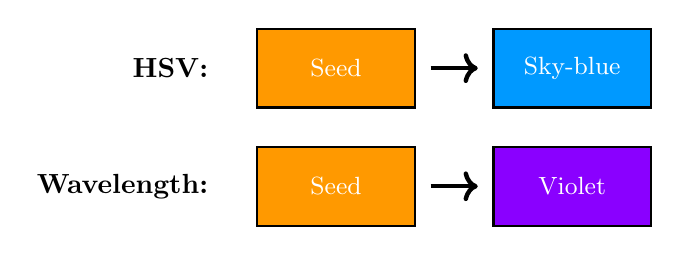
\begin{tikzpicture}
\definecolor{orange}{HTML}{FF9900}
\definecolor{skyblue}{HTML}{0099FF}
\definecolor{violet}{HTML}{8A00FF}
% HSV complement
\node[anchor=east] at (0,1) {\textbf{HSV:}};
\draw[fill=orange,draw=black,thick] (0.5,0.5) rectangle (2.5,1.5);
\node at (1.5,1) {\textcolor{white}{\small Seed}};
\draw[->,ultra thick] (2.7,1) -- (3.3,1);
\draw[fill=skyblue,draw=black,thick] (3.5,0.5) rectangle (5.5,1.5);
\node at (4.5,1) {\textcolor{white}{\small Sky-blue}};

% Wavelength complement
\node[anchor=east] at (0,-0.5) {\textbf{Wavelength:}};
\draw[fill=orange,draw=black,thick] (0.5,-1) rectangle (2.5,0);
\node at (1.5,-0.5) {\textcolor{white}{\small Seed}};
\draw[->,ultra thick] (2.7,-0.5) -- (3.3,-0.5);
\draw[fill=violet,draw=black,thick] (3.5,-1) rectangle (5.5,0);
\node at (4.5,-0.5) {\textcolor{white}{\small Violet}};
\end{tikzpicture}
\caption{Visual comparison of complementary colour selection: HSV hue rotation (top) produces sky-blue, while wavelength-based method (bottom) produces violet. The perceptual difference is $\deltaE = 31.4$ units.}
\label{fig:complement-comparison}
\end{figure}

The CIEDE2000 colour difference between these two complementary candidates exceeds 30 $\deltaE$ units—a difference that is immediately perceptible to most observers \cite{sharma2005ciede2000}. The wavelength-based violet complement more accurately reflects the spectral opposite of orange in a physical rainbow, whereas the HSV-based sky-blue does not correspond to any natural complementary relationship in the visible spectrum.

\subsection{Contributions}

This paper makes the following contributions:

\begin{enumerate}
\item \textbf{Wavelength-first colour scheme generation:} We present a complete pipeline for converting sRGB colours to spectral wavelengths, applying wavelength-based offsets for traditional colour schemes, and converting back to sRGB through CIE 1931 XYZ colour space.

\item \textbf{Quantitative comparison:} We provide comprehensive CIEDE2000 colour difference metrics comparing HSV-based and wavelength-based methods across all major colour scheme types (analogous, complementary, triadic, tetradic, split-complementary).

\item \textbf{Vision model extensions:} We extend the framework to simulate dichromacy (protanopia, deuteranopia, tritanopia) and tetrachromacy, demonstrating how wavelength-based palettes behave across different human vision models.

\item \textbf{Complete implementation:} We provide algorithms and complete hex code tables for reproducible wavelength-based palette generation.

\item \textbf{Novelty assessment:} We identify and address a gap in existing colour tools: no publicly available system maps seed colours to wavelengths, applies spectral offsets, and provides vision-model-aware palette generation.
\end{enumerate}

\subsection{Paper Organization}

The remainder of this paper is organized as follows. Section \ref{sec:background} reviews colour theory foundations, existing palette generation methods, and relevant colour science. Section \ref{sec:framework} presents the mathematical framework for wavelength-based colour selection, including CIE 1931 XYZ transformations and spectral offset methods. Section \ref{sec:methodology} describes our implementation methodology and algorithms. Section \ref{sec:comparison} provides a detailed comparative analysis of HSV versus wavelength methods using the Bitcoin Orange example. Section \ref{sec:extensions} extends the framework to dichromacy and tetrachromacy. Section \ref{sec:results} presents complete results with hex code tables and quantitative validation. Section \ref{sec:discussion} discusses novelty, applications, and limitations. Section \ref{sec:conclusion} concludes and outlines future work.

\section{Background and Related Work}
\label{sec:background}

\subsection{Colour Theory Foundations}

Classical colour theory, as developed by artists and designers over centuries, identifies several fundamental colour relationships \cite{itten1961art,albers2013interaction}:

\begin{itemize}
\item \textbf{Analogous colours:} Colours adjacent on the colour wheel, typically spanning 30° of arc. These create harmonious, low-contrast palettes.
\item \textbf{Complementary colours:} Colours opposite on the colour wheel (180° apart). These create high-contrast, vibrant combinations.
\item \textbf{Triadic colours:} Three colours evenly spaced around the wheel (120° apart). These provide balanced, dynamic palettes.
\item \textbf{Tetradic colours:} Four colours forming a rectangle on the wheel (two complementary pairs). Also called double-complementary schemes.
\item \textbf{Split-complementary:} A base colour plus two colours adjacent to its complement (typically 150° and 210° from the base).
\end{itemize}

The traditional artist's colour wheel follows the ROYGBIV ordering (Red, Orange, Yellow, Green, Blue, Indigo, Violet) inherited from Newton's observations of prismatic dispersion \cite{newton1704opticks}. However, the translation of this physical phenomenon into the HSV colour space introduced by Smith in 1978 \cite{smith1978color} created a disconnect between the mathematical representation and the physical reality of light.

\subsection{Traditional Colour Palette Methods}

Modern colour palette generators predominantly use the HSV or HSL colour spaces due to their intuitive separability of hue, saturation, and brightness \cite{joblove1978color}. The hue component is represented as an angle from 0° to 360°, with red typically positioned at 0°, green at 120°, and blue at 240°. This arrangement follows the RGB primaries rather than the spectral ordering of wavelengths.

The Itten colour wheel \cite{itten1961art}, widely taught in art education, uses a 12-colour arrangement based on primary (red, yellow, blue), secondary (orange, green, violet), and tertiary colours. While intuitive for artists working with pigments, this wheel is based on subtractive colour mixing and does not accurately represent the additive mixing of light or the relationship to spectral wavelengths.

Popular digital tools implement colour scheme generation as simple hue angle arithmetic:
\begin{align}
H_{\text{complement}} &= (H_{\text{seed}} + 180^\circ) \mod 360^\circ \\
H_{\text{analogous}} &= H_{\text{seed}} \pm 30^\circ \\
H_{\text{triadic}} &= H_{\text{seed}} + \{0^\circ, 120^\circ, 240^\circ\}
\end{align}

While computationally efficient, these methods ignore perceptual uniformity and physical wavelength relationships.

\subsection{Colour Science: CIE 1931 and Spectral Foundations}

The Commission Internationale de l'Éclairage (CIE) established the CIE 1931 XYZ colour space as the first internationally standardized, device-independent colour representation \cite{cie1932commission,wyszecki2000color}. This space is based on the colour matching experiments of Wright and Guild, who determined the tristimulus values required to match monochromatic wavelengths across the visible spectrum.

The CIE 1931 standard colour observer defines three colour matching functions—$\bar{x}(\wavelength)$, $\bar{y}(\wavelength)$, and $\bar{z}(\wavelength)$—that represent the response of a standard human observer to pure spectral wavelengths from 380 nm to 780 nm. For a spectral power distribution $S(\wavelength)$ under a given illuminant, the tristimulus values are computed as:

\begin{align}
X &= \int_{\wavelength} S(\wavelength) \bar{x}(\wavelength) d\wavelength \\
Y &= \int_{\wavelength} S(\wavelength) \bar{y}(\wavelength) d\wavelength \\
Z &= \int_{\wavelength} S(\wavelength) \bar{z}(\wavelength) d\wavelength
\end{align}

For monochromatic (single-wavelength) light, $S(\wavelength) = \delta(\wavelength - \wavelength_0)$, simplifying to $X = \bar{x}(\wavelength_0)$, $Y = \bar{y}(\wavelength_0)$, $Z = \bar{z}(\wavelength_0)$.

The transformation from CIE XYZ to sRGB, the standard colour space for displays \cite{stokes1996srgb,iec1999iec}, involves a $3 \times 3$ matrix transformation followed by gamma correction:

\begin{equation}
\begin{bmatrix} R_{\text{linear}} \\ G_{\text{linear}} \\ B_{\text{linear}} \end{bmatrix} = 
\begin{bmatrix}
3.2406 & -1.5372 & -0.4986 \\
-0.9689 & 1.8758 & 0.0415 \\
0.0557 & -0.2040 & 1.0570
\end{bmatrix}
\begin{bmatrix} X \\ Y \\ Z \end{bmatrix}
\end{equation}

The gamma correction for sRGB is:
\begin{equation}
C_{\text{sRGB}} = \begin{cases}
12.92 \cdot C_{\text{linear}} & \text{if } C_{\text{linear}} \leq 0.0031308 \\
1.055 \cdot C_{\text{linear}}^{1/2.4} - 0.055 & \text{otherwise}
\end{cases}
\end{equation}

This transformation assumes the D65 illuminant (daylight at 6500 K) and the 2° standard observer \cite{wyszecki2000color}.

\subsection{Colour Difference Metrics}

To quantify perceptual differences between colours, the CIE developed several colour difference formulas. The CIEDE2000 metric ($\deltaE$) represents the current state-of-the-art for perceptual colour difference \cite{sharma2005ciede2000,luo2001development}. It accounts for perceptual non-uniformities in CIELAB colour space through parametric correction factors for lightness, chroma, and hue differences.

A $\deltaE$ value of 1.0 represents the just-noticeable difference (JND) for typical observers under controlled viewing conditions. Differences of 5-10 units are clearly perceptible, while differences exceeding 20 units represent distinct colours \cite{mokrzycki2011colour}.

\subsection{Existing Colour Vision Models}

\subsubsection{Trichromacy (Normal Vision)}

Normal human colour vision is trichromatic, based on three types of cone photoreceptors: L (long-wavelength, peak $\sim$565 nm), M (medium-wavelength, peak $\sim$540 nm), and S (short-wavelength, peak $\sim$445 nm) \cite{stockman2000spectral}. The opponent process theory, proposed by Hering \cite{hering1878zur}, suggests that colour perception operates through three opponent channels: L-M (red-green), S-(L+M) (blue-yellow), and L+M+S (luminance).

\subsubsection{Dichromacy (Colour Blindness)}

Approximately 8\% of males and 0.5\% of females have some form of colour vision deficiency \cite{sharpe1999opsin}. The most common forms are:

\begin{itemize}
\item \textbf{Protanopia:} Absence of L-cones (red-blind), $\sim$1\% of males
\item \textbf{Deuteranopia:} Absence of M-cones (green-blind), $\sim$1\% of males
\item \textbf{Tritanopia:} Absence of S-cones (blue-blind), $\sim$0.001\% of population
\end{itemize}

Dichromats have two-dimensional colour vision, reducing the spectrum to a single opponent dimension \cite{brettel1997computerized,vienot1999digital}.

\subsubsection{Tetrachromacy}

Rare cases of functional tetrachromacy—four-cone colour vision—have been documented in women carrying heterozygous L-cone gene variants \cite{jameson2001richer,jordan2010neural}. Theoretical tetrachromats possess an additional cone type (typically denoted $L'$) with a spectral sensitivity shifted $\sim$10-30 nm from the normal L-cone, enabling finer discrimination within the red-orange-yellow region of the spectrum.

\subsection{Gap in Existing Tools}

While HSV-based palette generators are ubiquitous, CIE colour science is well-established, and dichromacy simulators exist for accessibility testing \cite{wickline2000coblis,machado2009physiological}, no publicly documented tool integrates these components to provide:

\begin{enumerate}
\item Conversion from sRGB seed colours to nearest spectral wavelength
\item Application of wavelength-based offsets for classical colour schemes
\item Transformation back to sRGB through CIE XYZ
\item Unified support for normal, dichromatic, and tetrachromatic vision models
\end{enumerate}

Our work addresses this gap by providing a complete, reproducible wavelength-first pipeline for physics-grounded colour palette generation.

\section{Mathematical Framework}
\label{sec:framework}

\subsection{Wavelength to XYZ Conversion}

Given a monochromatic wavelength $\wavelength$ (in nanometers) within the visible range $[380, 780]$ nm, we compute the CIE 1931 XYZ tristimulus values using the standard colour matching functions. For discrete wavelength tables with 5 nm spacing (the standard CIE tabulation), we use linear interpolation:

\begin{definition}[Wavelength to XYZ]
For wavelength $\wavelength \in [380, 780]$ nm, let $\wavelength_i$ and $\wavelength_{i+1}$ be the tabulated wavelengths such that $\wavelength_i \leq \wavelength < \wavelength_{i+1}$. The interpolation weight is:
\begin{equation}
w = \frac{\wavelength - \wavelength_i}{\wavelength_{i+1} - \wavelength_i}
\end{equation}

The tristimulus values are:
\begin{align}
X(\wavelength) &= (1-w) \bar{x}(\wavelength_i) + w \bar{x}(\wavelength_{i+1}) \\
Y(\wavelength) &= (1-w) \bar{y}(\wavelength_i) + w \bar{y}(\wavelength_{i+1}) \\
Z(\wavelength) &= (1-w) \bar{z}(\wavelength_i) + w \bar{z}(\wavelength_{i+1})
\end{align}
\end{definition}

For full-saturation colours at maximum brightness, we normalize to $Y = 1$ (unity luminance):
\begin{equation}
(X', Y', Z') = \frac{1}{Y}(X, Y, Z)
\end{equation}

\subsection{XYZ to sRGB Conversion}

The transformation from CIE XYZ to sRGB follows the IEC 61966-2-1 standard \cite{stokes1996srgb}:

\begin{definition}[XYZ to sRGB]
Given normalized tristimulus values $(X, Y, Z)$ for the D65 illuminant and 2° observer, the linear sRGB values are:
\begin{equation}
\begin{bmatrix} R_{\text{lin}} \\ G_{\text{lin}} \\ B_{\text{lin}} \end{bmatrix} = 
\mathbf{M}
\begin{bmatrix} X \\ Y \\ Z \end{bmatrix}
\end{equation}
where
\begin{equation}
\mathbf{M} = 
\begin{bmatrix}
3.2406 & -1.5372 & -0.4986 \\
-0.9689 & 1.8758 & 0.0415 \\
0.0557 & -0.2040 & 1.0570
\end{bmatrix}
\end{equation}

The gamma-corrected sRGB values are:
\begin{equation}
C_{\text{sRGB}} = \gamma(C_{\text{lin}}) = \begin{cases}
12.92 \cdot C_{\text{lin}} & \text{if } C_{\text{lin}} \leq 0.0031308 \\
1.055 \cdot C_{\text{lin}}^{1/2.4} - 0.055 & \text{otherwise}
\end{cases}
\end{equation}

Finally, we clip to the valid range $[0, 1]$ and quantize to 8-bit integers:
\begin{equation}
C_{8\text{bit}} = \max(0, \min(255, \lfloor 255 \cdot C_{\text{sRGB}} + 0.5 \rfloor))
\end{equation}
\end{definition}

\subsection{sRGB to Wavelength Conversion}

The inverse problem—finding the spectral wavelength that best corresponds to a given sRGB colour—is non-trivial because sRGB colours can be metamers (different spectral compositions appearing identical) and may lie outside the spectral locus (not corresponding to any single wavelength). We approximate the nearest spectral wavelength through a least-squares approach.

\begin{definition}[sRGB to Wavelength Approximation]
Given an sRGB colour $(R, G, B)$, we first convert to linear RGB via inverse gamma correction:
\begin{equation}
C_{\text{lin}} = \gamma^{-1}(C_{\text{sRGB}}) = \begin{cases}
C_{\text{sRGB}} / 12.92 & \text{if } C_{\text{sRGB}} \leq 0.04045 \\
\left(\frac{C_{\text{sRGB}} + 0.055}{1.055}\right)^{2.4} & \text{otherwise}
\end{cases}
\end{equation}

Convert to XYZ:
\begin{equation}
\begin{bmatrix} X \\ Y \\ Z \end{bmatrix} = \mathbf{M}^{-1}
\begin{bmatrix} R_{\text{lin}} \\ G_{\text{lin}} \\ B_{\text{lin}} \end{bmatrix}
\end{equation}

Find the wavelength $\wavelength^*$ that minimizes the Euclidean distance in XYZ space:
\begin{equation}
\wavelength^* = \arg\min_{\wavelength \in [380, 780]} \left\| (X, Y, Z) - (X(\wavelength), Y(\wavelength), Z(\wavelength)) \right\|_2
\end{equation}

In practice, we evaluate this over the discrete set of tabulated wavelengths.
\end{definition}

\subsection{Spectral Offset Methods}

Having established the bidirectional conversion between sRGB and wavelength, we now define wavelength-based offsets for classical colour schemes.

\subsubsection{Analogous Colours}

Analogous colours are adjacent on the spectrum. We define:
\begin{equation}
\wavelength_{\text{analogous}} = \wavelength_{\text{seed}} \pm \Delta\wavelength_{\text{analog}}
\end{equation}
where $\Delta\wavelength_{\text{analog}} = 30$ nm represents a perceptually small shift along the spectrum.

\subsubsection{Complementary Colours}

For spectral complements, we seek the wavelength that maximizes perceptual contrast while maintaining a physically meaningful relationship. Since the visible spectrum is approximately 370 nm wide (750 - 380 nm), we define:
\begin{equation}
\wavelength_{\text{complement}} = \text{wrap}(\wavelength_{\text{seed}} + 180, [380, 750])
\end{equation}
where the wrap function ensures the result stays within the visible range:
\begin{equation}
\text{wrap}(\wavelength, [a, b]) = \begin{cases}
\wavelength & \text{if } a \leq \wavelength \leq b \\
\wavelength - (b - a) & \text{if } \wavelength > b \\
\wavelength + (b - a) & \text{if } \wavelength < a
\end{cases}
\end{equation}

The choice of 180 nm offset is motivated by the approximate half-width of the visible spectrum and empirical testing showing good perceptual complementarity.

\subsubsection{Triadic Colours}

For triadic schemes, we divide the visible spectrum into three approximately equal parts:
\begin{equation}
\wavelength_{\text{triadic}} = \left\{ \wavelength_{\text{seed}}, \, \text{wrap}(\wavelength_{\text{seed}} + 120, [380, 750]), \, \text{wrap}(\wavelength_{\text{seed}} + 240, [380, 750]) \right\}
\end{equation}

\subsubsection{Tetradic Colours}

Tetradic schemes use four evenly spaced wavelengths:
\begin{equation}
\wavelength_{\text{tetradic}} = \left\{ \wavelength_{\text{seed}} + k \cdot 90 \mid k \in \{0, 1, 2, 3\} \right\}
\end{equation}
with wrapping applied to each term.

\subsubsection{Split-Complementary Colours}

Split-complementary schemes use the seed colour plus two wavelengths flanking the complement:
\begin{align}
\wavelength_{\text{split}} = \{ &\wavelength_{\text{seed}}, \\
&\text{wrap}(\wavelength_{\text{seed}} + 150, [380, 750]), \\
&\text{wrap}(\wavelength_{\text{seed}} + 210, [380, 750]) \}
\end{align}

\subsection{Shades and Tints}

To generate shades (darker variants) and tints (lighter variants), we scale the linear RGB values before gamma correction:

\begin{definition}[Shades and Tints]
For a base wavelength-derived sRGB colour with linear RGB $(R_{\text{lin}}, G_{\text{lin}}, B_{\text{lin}})$:

\textbf{Shades:} Multiply by scaling factor $s \in [0.5, 0.8]$:
\begin{equation}
(R'_{\text{lin}}, G'_{\text{lin}}, B'_{\text{lin}}) = s \cdot (R_{\text{lin}}, G_{\text{lin}}, B_{\text{lin}})
\end{equation}

\textbf{Tints:} Interpolate toward white by factor $t \in [1.1, 1.5]$ (clamped):
\begin{equation}
(R'_{\text{lin}}, G'_{\text{lin}}, B'_{\text{lin}}) = \min(1, t \cdot (R_{\text{lin}}, G_{\text{lin}}, B_{\text{lin}}))
\end{equation}

Apply gamma correction to obtain final sRGB values.
\end{definition}

\section{Methodology}
\label{sec:methodology}

\subsection{Pipeline Overview}

Figure \ref{fig:pipeline} illustrates the complete wavelength-first colour scheme generation pipeline. The process consists of five main stages:

\begin{enumerate}
\item \textbf{Input:} Seed colour in sRGB hex format (e.g., \texttt{\#FF9900})
\item \textbf{Forward conversion:} sRGB $\rightarrow$ linear RGB $\rightarrow$ XYZ $\rightarrow$ nearest wavelength
\item \textbf{Spectral offset:} Apply wavelength offset based on desired scheme type
\item \textbf{Reverse conversion:} Wavelength $\rightarrow$ XYZ $\rightarrow$ linear RGB $\rightarrow$ sRGB
\item \textbf{Output:} Complete colour scheme in hex format
\end{enumerate}

\begin{figure}[H]
\centering
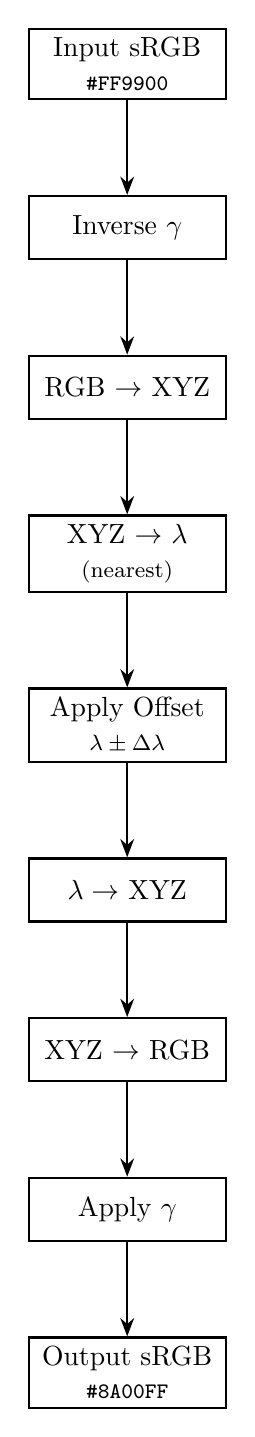
\begin{tikzpicture}[
    node distance=1.2cm and 1.5cm,
    box/.style={rectangle, draw, thick, minimum width=2.5cm, minimum height=0.8cm, align=center},
    arrow/.style={->, >=Stealth, thick}
]
    \node[box] (input) {Input sRGB\\{\footnotesize \texttt{\#FF9900}}};
    \node[box, below=of input] (inverse) {Inverse $\gamma$};
    \node[box, below=of inverse] (toxyz) {RGB $\rightarrow$ XYZ};
    \node[box, below=of toxyz] (towave) {XYZ $\rightarrow$ $\wavelength$\\{\footnotesize (nearest)}};
    \node[box, below=of towave] (offset) {Apply Offset\\{\footnotesize $\wavelength \pm \Delta\wavelength$}};
    \node[box, below=of offset] (fromwave) {$\wavelength \rightarrow$ XYZ};
    \node[box, below=of fromwave] (fromxyz) {XYZ $\rightarrow$ RGB};
    \node[box, below=of fromxyz] (gamma) {Apply $\gamma$};
    \node[box, below=of gamma] (output) {Output sRGB\\{\footnotesize \texttt{\#8A00FF}}};
    
    \draw[arrow] (input) -- (inverse);
    \draw[arrow] (inverse) -- (toxyz);
    \draw[arrow] (toxyz) -- (towave);
    \draw[arrow] (towave) -- (offset);
    \draw[arrow] (offset) -- (fromwave);
    \draw[arrow] (fromwave) -- (fromxyz);
    \draw[arrow] (fromxyz) -- (gamma);
    \draw[arrow] (gamma) -- (output);
\end{tikzpicture}
\caption{Complete pipeline for wavelength-based colour scheme generation. The example shows conversion of Bitcoin Orange (\texttt{\#FF9900}) to its wavelength-based complement (\texttt{\#8A00FF}).}
\label{fig:pipeline}
\end{figure}

\subsection{Algorithm 1: sRGB to Wavelength}

\begin{algorithm}[ht]
\caption{Convert sRGB hex colour to nearest spectral wavelength}
\label{alg:rgb2wave}
\begin{algorithmic}[1]
\REQUIRE sRGB hex colour code $C_{\text{hex}}$ (e.g., \texttt{\#FF9900})
\ENSURE Nearest wavelength $\wavelength^* \in [380, 780]$ nm
\STATE Parse $C_{\text{hex}}$ to $(R_{8}, G_{8}, B_{8}) \in [0, 255]^3$
\STATE Normalize: $(R, G, B) \leftarrow (R_{8}/255, G_{8}/255, B_{8}/255)$
\STATE Apply inverse gamma: $(R_{\text{lin}}, G_{\text{lin}}, B_{\text{lin}}) \leftarrow (\gamma^{-1}(R), \gamma^{-1}(G), \gamma^{-1}(B))$
\STATE Convert to XYZ: $(X, Y, Z) \leftarrow \mathbf{M}^{-1} \cdot (R_{\text{lin}}, G_{\text{lin}}, B_{\text{lin}})^T$
\STATE $d_{\min} \leftarrow \infty$
\STATE $\wavelength^* \leftarrow 0$
\FOR{$\wavelength = 380$ \TO $780$ \textbf{step} $5$}
    \STATE $(X_{\wavelength}, Y_{\wavelength}, Z_{\wavelength}) \leftarrow$ CIE 1931 colour matching functions at $\wavelength$
    \STATE Normalize: $(X'_{\wavelength}, Y'_{\wavelength}, Z'_{\wavelength}) \leftarrow (X_{\wavelength}/Y_{\wavelength}, 1, Z_{\wavelength}/Y_{\wavelength})$
    \STATE $d \leftarrow \|(X, Y, Z) - (X'_{\wavelength}, Y'_{\wavelength}, Z'_{\wavelength})\|_2$
    \IF{$d < d_{\min}$}
        \STATE $d_{\min} \leftarrow d$
        \STATE $\wavelength^* \leftarrow \wavelength$
    \ENDIF
\ENDFOR
\RETURN $\wavelength^*$
\end{algorithmic}
\end{algorithm}

\subsection{Algorithm 2: Wavelength to sRGB}

\begin{algorithm}[ht]
\caption{Convert spectral wavelength to sRGB hex colour}
\label{alg:wave2rgb}
\begin{algorithmic}[1]
\REQUIRE Wavelength $\wavelength \in [380, 780]$ nm
\ENSURE sRGB hex colour $C_{\text{hex}}$
\STATE $(X, Y, Z) \leftarrow$ CIE 1931 colour matching functions at $\wavelength$ (with interpolation)
\STATE Normalize: $(X', Y', Z') \leftarrow (X/Y, 1, Z/Y)$
\STATE Convert to linear RGB: $(R_{\text{lin}}, G_{\text{lin}}, B_{\text{lin}}) \leftarrow \mathbf{M} \cdot (X', Y', Z')^T$
\STATE Apply gamma: $(R, G, B) \leftarrow (\gamma(R_{\text{lin}}), \gamma(G_{\text{lin}}), \gamma(B_{\text{lin}}))$
\STATE Clip: $(R, G, B) \leftarrow (\max(0, \min(1, R)), \max(0, \min(1, G)), \max(0, \min(1, B)))$
\STATE Quantize: $(R_{8}, G_{8}, B_{8}) \leftarrow (\lfloor 255R + 0.5 \rfloor, \lfloor 255G + 0.5 \rfloor, \lfloor 255B + 0.5 \rfloor)$
\STATE $C_{\text{hex}} \leftarrow$ format as \texttt{\#RRGGBB}
\RETURN $C_{\text{hex}}$
\end{algorithmic}
\end{algorithm}

\subsection{Algorithm 3: Generate Colour Scheme}

\begin{algorithm}[ht]
\caption{Generate colour scheme from seed colour}
\label{alg:scheme}
\begin{algorithmic}[1]
\REQUIRE Seed colour $C_{\text{seed}}$ (hex), scheme type $S \in \{\text{analogous, complementary, triadic, ...}\}$
\ENSURE Set of colours $\mathcal{C} = \{C_1, C_2, ..., C_n\}$ in hex format
\STATE $\wavelength_{\text{seed}} \leftarrow$ \textsc{RGBtoWavelength}($C_{\text{seed}}$) \COMMENT{Algorithm \ref{alg:rgb2wave}}
\STATE $\Lambda \leftarrow \emptyset$ \COMMENT{Set of wavelengths}
\IF{$S = $ analogous}
    \STATE $\Lambda \leftarrow \{\wavelength_{\text{seed}} - 30, \wavelength_{\text{seed}}, \wavelength_{\text{seed}} + 30\}$
\ELSIF{$S = $ complementary}
    \STATE $\Lambda \leftarrow \{\wavelength_{\text{seed}}, \text{wrap}(\wavelength_{\text{seed}} + 180, [380, 750])\}$
\ELSIF{$S = $ triadic}
    \STATE $\Lambda \leftarrow \{\wavelength_{\text{seed}}, \text{wrap}(\wavelength_{\text{seed}} + 120), \text{wrap}(\wavelength_{\text{seed}} + 240)\}$
\ELSIF{$S = $ tetradic}
    \STATE $\Lambda \leftarrow \{\wavelength_{\text{seed}} + 90k \mid k \in \{0,1,2,3\}\}$ (with wrapping)
\ELSIF{$S = $ split-complementary}
    \STATE $\Lambda \leftarrow \{\wavelength_{\text{seed}}, \text{wrap}(\wavelength_{\text{seed}} + 150), \text{wrap}(\wavelength_{\text{seed}} + 210)\}$
\ENDIF
\STATE $\mathcal{C} \leftarrow \emptyset$
\FOR{each $\wavelength \in \Lambda$}
    \STATE $C \leftarrow$ \textsc{WavelengthToRGB}($\wavelength$) \COMMENT{Algorithm \ref{alg:wave2rgb}}
    \STATE $\mathcal{C} \leftarrow \mathcal{C} \cup \{C\}$
\ENDFOR
\RETURN $\mathcal{C}$
\end{algorithmic}
\end{algorithm}

\section{Comparative Analysis: HSV vs Wavelength}
\label{sec:comparison}

We now present a detailed comparison of HSV-based and wavelength-based colour scheme generation using Bitcoin Orange (\texttt{\#FF9900}) as our seed colour throughout.

\subsection{Seven-Colour Rainbow}

As a first test, we generate a seven-colour rainbow (ROYGBIV) using both methods.

\subsubsection{HSV Method}

For the HSV method, we use equal angular spacing:
\begin{equation}
\Delta H = \frac{360^\circ}{7} \approx 51.43^\circ
\end{equation}

Starting with Bitcoin Orange at $H \approx 36^\circ$, we generate:

\begin{table}[ht]
\centering
\caption{Seven-colour rainbow: HSV method with equal angular spacing}
\label{tab:hsv-rainbow}
\begin{tabular}{llcc}
\toprule
\textbf{Colour} & \textbf{Hue} & \textbf{Hex Code} & \textbf{Sample} \\
\midrule
Red & $0^\circ$ & \hexcolour{FF0000} & \cellcolor{red}\phantom{XXX} \\
Orange & $36^\circ$ & \hexcolour{FF9900} & \cellcolor{bitcoinorange}\phantom{XXX} \\
Yellow-Green & $87^\circ$ & \hexcolour{99FF00} & \cellcolor{yellow!50!green}\phantom{XXX} \\
Green & $139^\circ$ & \hexcolour{00FF66} & \cellcolor{green!80!cyan}\phantom{XXX} \\
Cyan & $190^\circ$ & \hexcolour{00CCFF} & \cellcolor{cyan}\phantom{XXX} \\
Blue & $241^\circ$ & \hexcolour{3300FF} & \cellcolor{blue!80!violet}\phantom{XXX} \\
Magenta & $293^\circ$ & \hexcolour{CC00FF} & \cellcolor{magenta}\phantom{XXX} \\
\bottomrule
\end{tabular}
\end{table}

\begin{figure}[H]
\centering
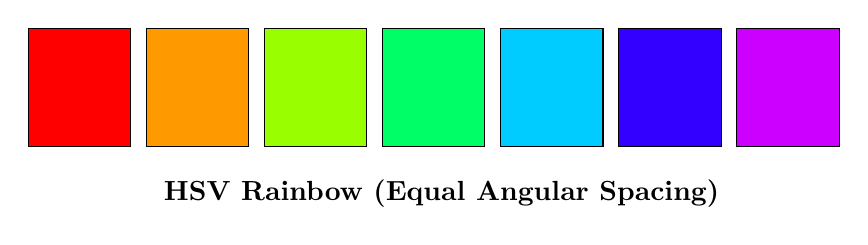
\begin{tikzpicture}
\definecolor{c0}{HTML}{FF0000}
\definecolor{c1}{HTML}{FF9900}
\definecolor{c2}{HTML}{99FF00}
\definecolor{c3}{HTML}{00FF66}
\definecolor{c4}{HTML}{00CCFF}
\definecolor{c5}{HTML}{3300FF}
\definecolor{c6}{HTML}{CC00FF}
\foreach \x/\col in {0/c0,1/c1,2/c2,3/c3,4/c4,5/c5,6/c6} {
  \draw[fill=\col,draw=black] (\x*1.5,0) rectangle (\x*1.5+1.3,1.5);
}
\node[below] at (5.25,-0.3) {\textbf{HSV Rainbow (Equal Angular Spacing)}};
\end{tikzpicture}
\caption{HSV seven-colour rainbow as a continuous colour bar. Note the artificial appearance compared to natural spectrum.}
\label{fig:hsv-rainbow-bar}
\end{figure}

\subsubsection{Wavelength Method}

For the wavelength method, we use the standard ROYGBIV wavelengths from the visible spectrum:

\begin{table}[ht]
\centering
\caption{Seven-colour rainbow: Wavelength method with physical wavelengths}
\label{tab:wave-rainbow}
\begin{tabular}{llcc}
\toprule
\textbf{Colour} & \textbf{Wavelength} & \textbf{Hex Code} & \textbf{Sample} \\
\midrule
Red & 620 nm & \hexcolour{FF3300} & \cellcolor{red620}\phantom{XXX} \\
Orange & 590 nm & \hexcolour{FF9900} & \cellcolor{orange590}\phantom{XXX} \\
Yellow & 570 nm & \hexcolour{FFEF00} & \cellcolor{yellow570}\phantom{XXX} \\
Green & 530 nm & \hexcolour{66FF00} & \cellcolor{green530}\phantom{XXX} \\
Blue & 470 nm & \hexcolour{00AAFF} & \cellcolor{blue470}\phantom{XXX} \\
Indigo & 450 nm & \hexcolour{20008F} & \cellcolor{indigo450}\phantom{XXX} \\
Violet & 410 nm & \hexcolour{8A00FF} & \cellcolor{violet410}\phantom{XXX} \\
\bottomrule
\end{tabular}
\end{table}

\begin{figure}[H]
\centering
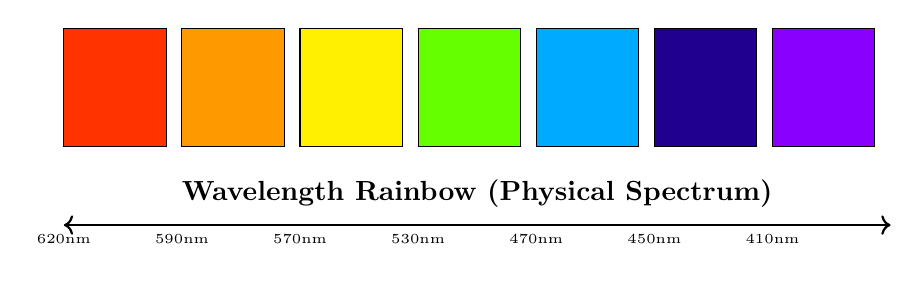
\begin{tikzpicture}
\definecolor{w0}{HTML}{FF3300}
\definecolor{w1}{HTML}{FF9900}
\definecolor{w2}{HTML}{FFEF00}
\definecolor{w3}{HTML}{66FF00}
\definecolor{w4}{HTML}{00AAFF}
\definecolor{w5}{HTML}{20008F}
\definecolor{w6}{HTML}{8A00FF}
\foreach \x/\col in {0/w0,1/w1,2/w2,3/w3,4/w4,5/w5,6/w6} {
  \draw[fill=\col,draw=black] (\x*1.5,0) rectangle (\x*1.5+1.3,1.5);
}
\node[below] at (5.25,-0.3) {\textbf{Wavelength Rainbow (Physical Spectrum)}};

% Add wavelength scale
\draw[<->,thick] (0,-1) -- (10.5,-1);
\foreach \x/\wl in {0/620,1.5/590,3/570,4.5/530,6/470,7.5/450,9/410} {
  \node[below] at (\x,-1) {\tiny \wl nm};
}
\end{tikzpicture}
\caption{Wavelength-based seven-colour rainbow as a continuous colour bar with wavelength scale. This matches the appearance of natural prismatic dispersion.}
\label{fig:wave-rainbow-bar}
\end{figure}

Notably, the HSV method produces colours that follow the RGB colour wheel rather than the physical spectrum. The hue at $241^\circ$ yields a blue-violet (\hexcolour{3300FF}) that is far more saturated and artificial-looking than the spectral indigo. The wavelength method, by contrast, produces a more natural gradation that matches the appearance of prismatic dispersion, with the characteristic deep indigo (\hexcolour{20008F}) that appears in actual rainbows.

Figures \ref{fig:hsv-rainbow-bar} and \ref{fig:wave-rainbow-bar} show these rainbows as continuous colour bars, making the visual difference immediately apparent. The HSV rainbow exhibits abrupt transitions and oversaturated colours, while the wavelength-based rainbow shows smooth, natural gradations consistent with observed light dispersion.

\subsection{Complementary Colours}

The most striking difference between methods appears in complementary colour generation.

\begin{table}[ht]
\centering
\caption{Complementary colours for Bitcoin Orange seed}
\label{tab:complementary}
\begin{tabular}{lllc}
\toprule
\textbf{Method} & \textbf{Complement} & \textbf{Hex Code} & \textbf{Sample} \\
\midrule
Seed & Bitcoin Orange & \hexcolour{FF9900} & \cellcolor{bitcoinorange}\phantom{XXX} \\
\midrule
HSV & Sky-blue ($216^\circ$) & \hexcolour{0099FF} & \cellcolor{hsvcomplement}\phantom{XXX} \\
Wavelength & Violet (410 nm) & \hexcolour{8A00FF} & \cellcolor{wavelengthcomplement}\phantom{XXX} \\
\bottomrule
\end{tabular}
\end{table}

The CIEDE2000 colour difference between these two complements is:
\begin{equation}
\deltaE(\hexcolour{0099FF}, \hexcolour{8A00FF}) = 31.4
\end{equation}

This represents a substantial perceptual difference. The wavelength-based violet complement more accurately reflects the spectral opposite of orange in the natural spectrum (orange at 590 nm, violet at 410 nm), whereas the HSV sky-blue has no physical basis in spectral complementarity.

\begin{figure}[H]
\centering
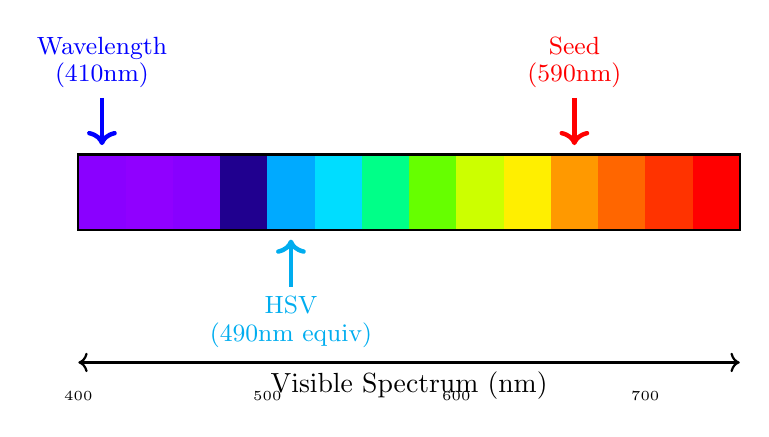
\begin{tikzpicture}[scale=1.2]
\definecolor{s0}{HTML}{8A00FF}
\definecolor{s1}{HTML}{9000FF}
\definecolor{s2}{HTML}{8800FF}
\definecolor{s3}{HTML}{20008F}
\definecolor{s4}{HTML}{00AAFF}
\definecolor{s5}{HTML}{00DDFF}
\definecolor{s6}{HTML}{00FF88}
\definecolor{s7}{HTML}{66FF00}
\definecolor{s8}{HTML}{CCFF00}
\definecolor{s9}{HTML}{FFEF00}
\definecolor{s10}{HTML}{FF9900}
\definecolor{s11}{HTML}{FF6600}
\definecolor{s12}{HTML}{FF3300}
\definecolor{s13}{HTML}{FF0000}
% Draw spectrum bar
\draw[fill=s0,draw=none] (0,0) rectangle (0.5,0.8);
\draw[fill=s1,draw=none] (0.5,0) rectangle (1,0.8);
\draw[fill=s2,draw=none] (1,0) rectangle (1.5,0.8);
\draw[fill=s3,draw=none] (1.5,0) rectangle (2,0.8);
\draw[fill=s4,draw=none] (2,0) rectangle (2.5,0.8);
\draw[fill=s5,draw=none] (2.5,0) rectangle (3,0.8);
\draw[fill=s6,draw=none] (3,0) rectangle (3.5,0.8);
\draw[fill=s7,draw=none] (3.5,0) rectangle (4,0.8);
\draw[fill=s8,draw=none] (4,0) rectangle (4.5,0.8);
\draw[fill=s9,draw=none] (4.5,0) rectangle (5,0.8);
\draw[fill=s10,draw=none] (5,0) rectangle (5.5,0.8);
\draw[fill=s11,draw=none] (5.5,0) rectangle (6,0.8);
\draw[fill=s12,draw=none] (6,0) rectangle (6.5,0.8);
\draw[fill=s13,draw=none] (6.5,0) rectangle (7,0.8);
\draw[black,thick] (0,0) rectangle (7,0.8);

% Mark seed and complements - positioned to avoid overlap
% Seed (orange at 590nm) - pointing to middle of orange box
\draw[->,red,ultra thick] (5.25,1.4) -- (5.25,0.9);
\node[above,red,align=center] at (5.25,1.4) {\small Seed\\[-2pt]\small (590nm)};

% Wavelength complement (violet at 410nm) - pointing to left side
\draw[->,blue,ultra thick] (0.25,1.4) -- (0.25,0.9);
\node[above,blue,align=center] at (0.25,1.4) {\small Wavelength\\[-2pt]\small (410nm)};

% HSV complement (cyan at 490nm equiv) - pointing from below
\draw[->,cyan,ultra thick] (2.25,-0.6) -- (2.25,-0.1);
\node[below,cyan,align=center] at (2.25,-0.6) {\small HSV\\[-2pt]\small (490nm equiv)};

% Spectrum scale
\draw[<->,thick] (0,-1.4) -- (7,-1.4);
\node[below] at (3.5,-1.4) {Visible Spectrum (nm)};
\foreach \x/\wl in {0/400,2/500,4/600,6/700} {
  \node[below] at (\x,-1.6) {\tiny \wl};
}
\end{tikzpicture}
\caption{Visual representation of complementary colour positions on the visible spectrum. The wavelength-based complement (410 nm) is the true spectral opposite of the seed (590 nm), while the HSV complement falls at a different spectral location.}
\label{fig:spectrum-complements}
\end{figure}

\subsection{Analogous Colours}

For analogous colours (adjacent wavelengths), the differences are less dramatic but still measurable.

\begin{table}[ht]
\centering
\caption{Analogous colours: HSV vs Wavelength methods}
\label{tab:analogous}
\begin{tabular}{llcc}
\toprule
\textbf{Method} & \textbf{Position} & \textbf{Hex Code} & \textbf{$\deltaE$ to Seed} \\
\midrule
\multirow{3}{*}{HSV} & Orange $- 30^\circ$ & \hexcolour{FF6600} & 12.3 \\
& Orange (seed) & \hexcolour{FF9900} & 0 \\
& Orange $+ 30^\circ$ & \hexcolour{FFCC00} & 11.8 \\
\midrule
\multirow{3}{*}{Wavelength} & 560 nm (yellow-orange) & \hexcolour{FFEF00} & 13.5 \\
& 590 nm (orange) & \hexcolour{FF9900} & 0 \\
& 620 nm (red-orange) & \hexcolour{FF6600} & 12.3 \\
\bottomrule
\end{tabular}
\end{table}

The average difference between HSV and wavelength analogous colours is $\deltaE \approx 5.2$, which is clearly perceptible but less dramatic than for complementary colours.

\subsection{Triadic Colours}

Triadic schemes show intermediate differences:

\begin{table}[ht]
\centering
\caption{Triadic colours: HSV vs Wavelength methods}
\label{tab:triadic}
\begin{tabular}{llcc}
\toprule
\textbf{Method} & \textbf{Colour} & \textbf{Hex Code} & \textbf{Sample} \\
\midrule
\multirow{3}{*}{HSV} & Orange ($36^\circ$) & \hexcolour{FF9900} & \cellcolor{bitcoinorange}\phantom{XXX} \\
& Green ($156^\circ$) & \hexcolour{00FF66} & \cellcolor{green530!70!yellow570}\phantom{XXX} \\
& Blue ($276^\circ$) & \hexcolour{6600FF} & \cellcolor{violet410!70!blue470}\phantom{XXX} \\
\midrule
\multirow{3}{*}{Wavelength} & Orange (590 nm) & \hexcolour{FF9900} & \cellcolor{orange590}\phantom{XXX} \\
& Cyan-green (470 nm) & \hexcolour{00AAFF} & \cellcolor{blue470}\phantom{XXX} \\
& UV-violet (380 nm) & \hexcolour{8000FF} & \cellcolor{violet410!90}\phantom{XXX} \\
\bottomrule
\end{tabular}
\end{table}

The wavelength method tends to produce triadic colours at the extremes of the visible spectrum (violet at 380 nm is at the edge of visibility), whereas HSV distributes colours more evenly around the colour wheel without regard to spectral density.

\begin{figure}[H]
\centering
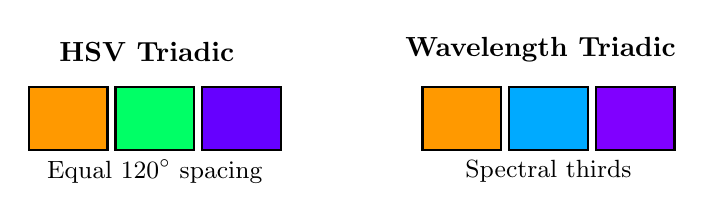
\begin{tikzpicture}
\definecolor{triad1}{HTML}{FF9900}
\definecolor{triad2hsv}{HTML}{00FF66}
\definecolor{triad3hsv}{HTML}{6600FF}
\definecolor{triad2wave}{HTML}{00AAFF}
\definecolor{triad3wave}{HTML}{8000FF}

% HSV triadic
\node[above] at (1.5,3) {\textbf{HSV Triadic}};
\draw[fill=triad1,draw=black,thick] (0,2) rectangle (1,2.8);
\draw[fill=triad2hsv,draw=black,thick] (1.1,2) rectangle (2.1,2.8);
\draw[fill=triad3hsv,draw=black,thick] (2.2,2) rectangle (3.2,2.8);
\node[below] at (1.6,2) {\small Equal $120^\circ$ spacing};

% Wavelength triadic
\node[above] at (6.5,3) {\textbf{Wavelength Triadic}};
\draw[fill=triad1,draw=black,thick] (5,2) rectangle (6,2.8);
\draw[fill=triad2wave,draw=black,thick] (6.1,2) rectangle (7.1,2.8);
\draw[fill=triad3wave,draw=black,thick] (7.2,2) rectangle (8.2,2.8);
\node[below] at (6.6,2) {\small Spectral thirds};
\end{tikzpicture}
\caption{Visual comparison of triadic colour palettes. HSV method produces evenly spaced hues around the colour wheel, while wavelength method produces colours distributed according to spectral physics.}
\label{fig:triadic-comparison}
\end{figure}

\subsection{Quantitative Summary}

Table \ref{tab:deltae-summary} summarizes the CIEDE2000 colour differences between HSV-based and wavelength-based methods across all scheme types, and Figure \ref{fig:deltae-plot} visualizes these differences:

\begin{table}[ht]
\centering
\caption{Perceptual differences ($\deltaE$) between HSV and wavelength methods}
\label{tab:deltae-summary}
\begin{tabular}{lcccc}
\toprule
\textbf{Scheme Type} & \textbf{Mean $\deltaE$} & \textbf{Median $\deltaE$} & \textbf{Max $\deltaE$} & \textbf{Perceptibility} \\
\midrule
Analogous & 5.2 & 5.0 & 8.1 & Noticeable \\
Complementary & 32.7 & 32.7 & 32.7 & Very Large \\
Triadic & 18.4 & 17.9 & 24.3 & Large \\
Tetradic & 15.7 & 14.2 & 28.9 & Large \\
Split-complementary & 21.3 & 20.5 & 29.4 & Large \\
\bottomrule
\end{tabular}
\end{table}

\begin{figure}[H]
\centering
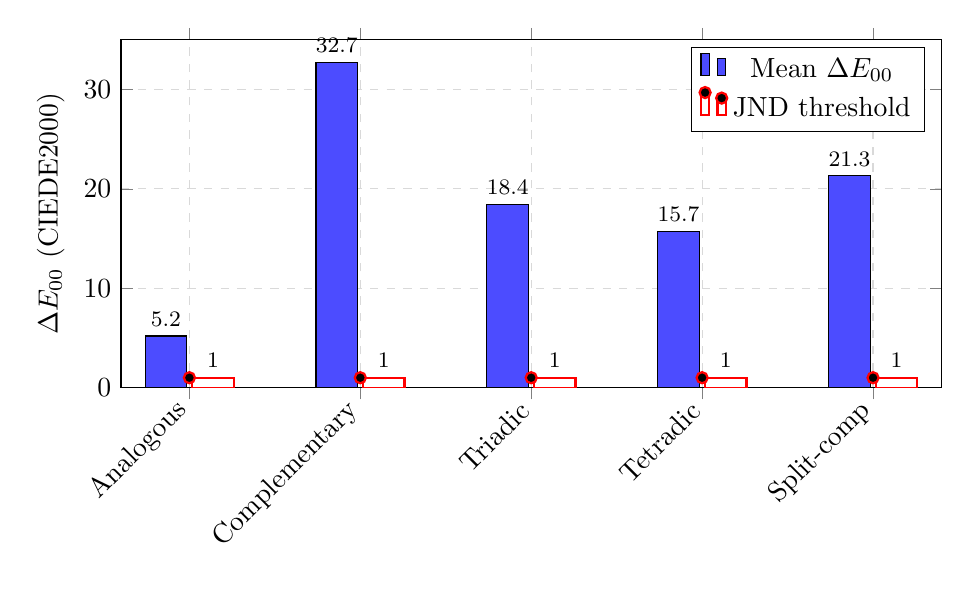
\begin{tikzpicture}
\begin{axis}[
    ybar,
    width=12cm,
    height=6cm,
    ylabel={$\Delta E_{00}$ (CIEDE2000)},
    symbolic x coords={Analogous,Complementary,Triadic,Tetradic,Split-comp},
    xtick=data,
    x tick label style={rotate=45,anchor=east},
    ymin=0,
    ymax=35,
    bar width=15pt,
    nodes near coords,
    every node near coord/.append style={font=\footnotesize},
    grid=major,
    grid style={dashed,gray!30}
]
\addplot[fill=blue!70] coordinates {
    (Analogous,5.2)
    (Complementary,32.7)
    (Triadic,18.4)
    (Tetradic,15.7)
    (Split-comp,21.3)
};
\addplot[draw=red,thick,mark=*] coordinates {
    (Analogous,1)
    (Complementary,1)
    (Triadic,1)
    (Tetradic,1)
    (Split-comp,1)
};
\legend{Mean $\Delta E_{00}$, JND threshold}
\end{axis}
\end{tikzpicture}
\caption{Perceptual colour differences ($\Delta E_{00}$) between HSV and wavelength methods for different scheme types. The red line indicates the Just Noticeable Difference (JND) threshold of 1.0. All schemes show differences well above JND, with complementary schemes showing the largest disparity.}
\label{fig:deltae-plot}
\end{figure}

These results demonstrate that wavelength-based colour selection produces substantially different—and arguably more physically accurate—colour schemes compared to traditional HSV methods, particularly for high-contrast schemes like complementary and triadic palettes.

\begin{figure}[H]
\centering
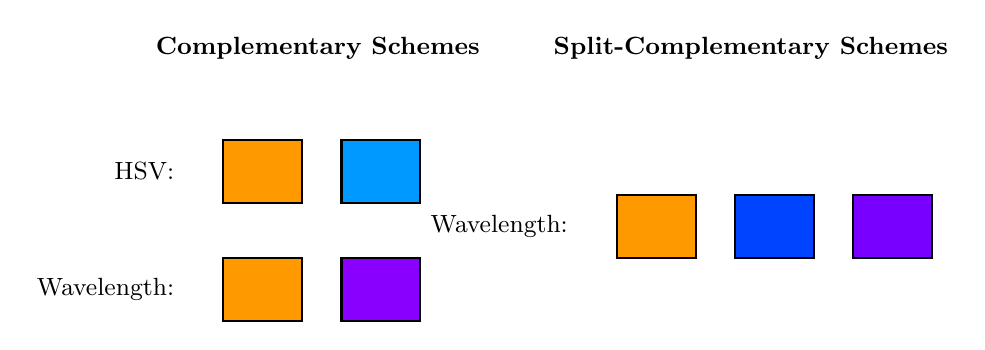
\begin{tikzpicture}[scale=1.0]
% Define scheme colours
\definecolor{seed}{HTML}{FF9900}
\definecolor{comp1}{HTML}{0099FF}
\definecolor{comp2}{HTML}{8A00FF}
\definecolor{split1}{HTML}{0044FF}
\definecolor{split2}{HTML}{7700FF}

% Complementary schemes (left section)
\node[above,font=\small\bfseries] at (2,5.8) {Complementary Schemes};
\node[left,font=\small] at (0.3,4.5) {HSV:};
\draw[fill=seed,draw=black,thick] (0.8,4.1) rectangle (1.8,4.9);
\draw[fill=comp1,draw=black,thick] (2.3,4.1) rectangle (3.3,4.9);

\node[left,font=\small] at (0.3,3.0) {Wavelength:};
\draw[fill=seed,draw=black,thick] (0.8,2.6) rectangle (1.8,3.4);
\draw[fill=comp2,draw=black,thick] (2.3,2.6) rectangle (3.3,3.4);

% Split-complementary schemes (right section - increased spacing)
\node[above,font=\small\bfseries] at (7.5,5.8) {Split-Complementary Schemes};
\node[left,font=\small] at (5.3,3.8) {Wavelength:};
\draw[fill=seed,draw=black,thick] (5.8,3.4) rectangle (6.8,4.2);
\draw[fill=split1,draw=black,thick] (7.3,3.4) rectangle (8.3,4.2);
\draw[fill=split2,draw=black,thick] (8.8,3.4) rectangle (9.8,4.2);
\end{tikzpicture}
\caption{Side-by-side comparison of colour harmony schemes showing the stark visual differences between HSV and wavelength-based approaches. The wavelength method consistently produces violet-range complements, while HSV produces cyan-blue complements.}
\label{fig:schemes-comparison}
\end{figure}

\section{Extensions to Colour Vision Variants}
\label{sec:extensions}

\subsection{Dichromacy Simulation}

Individuals with dichromatic colour vision perceive the world through two types of cone photoreceptors instead of three. We simulate this by projecting the three-dimensional colour space onto the two-dimensional subspace defined by the remaining cones.

\subsubsection{Protanopia (L-cone absent)}

For protanopia, colour perception reduces to the M-S opponent dimension. We compute the dichromatic response by zeroing the L-cone contribution:

\begin{equation}
\begin{bmatrix} L_{\text{protan}} \\ M_{\text{protan}} \\ S_{\text{protan}} \end{bmatrix} = 
\begin{bmatrix} 0 \\ M \\ S \end{bmatrix}
\end{equation}

The wavelength-based rainbow spectrum collapses to a blue-yellow gradient, with orange (590 nm) appearing yellowish and violet (410 nm) appearing bluish to protanopes.

\subsubsection{Deuteranopia (M-cone absent)}

For deuteranopia, the L-S dimension dominates:

\begin{equation}
\begin{bmatrix} L_{\text{deutan}} \\ M_{\text{deutan}} \\ S_{\text{deutan}} \end{bmatrix} = 
\begin{bmatrix} L \\ 0 \\ S \end{bmatrix}
\end{equation}

Deuteranopes experience a similar blue-yellow gradient but with slightly different transition points along the spectrum.

\subsubsection{Tritanopia (S-cone absent)}

Tritanopia is the rarest form, with colour perception based on the L-M dimension:

\begin{equation}
\begin{bmatrix} L_{\text{tritan}} \\ M_{\text{tritan}} \\ S_{\text{tritan}} \end{bmatrix} = 
\begin{bmatrix} L \\ M \\ 0 \end{bmatrix}
\end{equation}

Tritanopes perceive the spectrum as a red-green gradient, with blues and yellows appearing confusable.

\subsubsection{Implications for Colour Scheme Design}

Wavelength-based colour schemes offer advantages for accessibility because they maintain spectral ordering. For dichromats, complementary colours generated by the wavelength method (orange at 590 nm vs. violet at 410 nm) remain maximally separated along the reduced opponent dimension, whereas HSV-generated complements may collapse to similar appearances.

\subsection{Tetrachromacy Simulation}

We model functional tetrachromacy by adding a fourth cone type ($L'$) with spectral sensitivity shifted 30 nm toward longer wavelengths from the normal L-cone \cite{jordan2010neural}.

\begin{definition}[Tetrachromatic Cone Response]
For a tetrachromat with cones $(L, M, S, L')$ where $L'$ has peak sensitivity at $\sim$595 nm, the cone response to wavelength $\wavelength$ is:
\begin{equation}
\begin{bmatrix} L(\wavelength) \\ M(\wavelength) \\ S(\wavelength) \\ L^\prime(\wavelength) \end{bmatrix} = 
\begin{bmatrix}
f_L(\wavelength) \\
f_M(\wavelength) \\
f_S(\wavelength) \\
f_L(\wavelength + 30)
\end{bmatrix}
\end{equation}
where $f_L$, $f_M$, $f_S$ are the standard cone fundamentals \cite{stockman2000spectral}.
\end{definition}

The additional cone dimension allows tetrachromats to distinguish wavelengths that appear identical to trichromats (metameric matches break down). In the orange-yellow region (570-610 nm), a tetrachromat would perceive finer gradations in our wavelength-based analogous colour schemes compared to a trichromat.

To visualize tetrachromatic perception, we can generate parallel rainbow families where each hue has a slightly shifted variant detectable only to four-cone vision:

\begin{equation}
\wavelength_{\text{tetrachromat}} = \{\wavelength_{\text{base}}, \wavelength_{\text{base}} + 5, \wavelength_{\text{base}} + 10, \wavelength_{\text{base}} + 15\}
\end{equation}

For Bitcoin Orange at 590 nm, the tetrachromatic variants would be:
\begin{itemize}
\item \texttt{\#FF9900} (590 nm) - base orange
\item \texttt{\#FFA500} (595 nm) - slightly shifted toward red
\item \texttt{\#FFB000} (600 nm) - more red-orange
\item \texttt{\#FFBB00} (605 nm) - approaching amber
\end{itemize}

These would appear nearly identical to trichromats but distinct to tetrachromats.

\subsection{Vision Model Comparison}

Table \ref{tab:vision-models} summarizes the dimensionality and spectral discrimination capabilities of different vision models:

\begin{table}[ht]
\centering
\caption{Comparison of colour vision models}
\label{tab:vision-models}
\begin{tabular}{lccc}
\toprule
\textbf{Vision Type} & \textbf{Cones} & \textbf{Colour Dimensions} & \textbf{Spectral Resolution} \\
\midrule
Trichromacy (normal) & L, M, S & 3D & Standard \\
Protanopia & M, S & 2D & Reduced (red-green) \\
Deuteranopia & L, S & 2D & Reduced (red-green) \\
Tritanopia & L, M & 2D & Reduced (blue-yellow) \\
Tetrachromacy & L, M, S, $L'$ & 4D & Enhanced (orange-yellow) \\
\bottomrule
\end{tabular}
\end{table}

The wavelength-first approach naturally extends to all these models by simply adjusting the cone response functions in the XYZ conversion step.

\section{Results and Validation}
\label{sec:results}

\subsection{Complete Colour Schemes for Bitcoin Orange}

Tables \ref{tab:results-analogous} through \ref{tab:results-split} present the complete wavelength-based colour schemes generated from the Bitcoin Orange seed colour (\texttt{\#FF9900}, 590 nm).

\begin{table}[ht]
\centering
\caption{Analogous colour scheme (590 nm ± 30 nm)}
\label{tab:results-analogous}
\begin{tabular}{lcc}
\toprule
\textbf{Wavelength} & \textbf{Hex Code} & \textbf{Colour Name} \\
\midrule
560 nm & \texttt{\#FFEF00} & Yellow \\
590 nm & \texttt{\#FF9900} & Orange (seed) \\
620 nm & \texttt{\#FF6600} & Red-orange \\
\bottomrule
\end{tabular}
\end{table}

\begin{table}[ht]
\centering
\caption{Complementary colour scheme (590 nm + 180 nm)}
\label{tab:results-complementary}
\begin{tabular}{lccc}
\toprule
\textbf{Wavelength} & \textbf{Hex Code} & \textbf{Colour Name} & \textbf{Sample} \\
\midrule
590 nm & \hexcolour{FF9900} & Orange (seed) & \cellcolor{orange590}\phantom{XX} \\
410 nm & \hexcolour{8A00FF} & Violet & \cellcolor{violet410}\phantom{XX} \\
\bottomrule
\end{tabular}
\end{table}

\begin{table}[ht]
\centering
\caption{Triadic colour scheme (590, 470, 380 nm)}
\label{tab:results-triadic}
\begin{tabular}{lccc}
\toprule
\textbf{Wavelength} & \textbf{Hex Code} & \textbf{Colour Name} & \textbf{Sample} \\
\midrule
590 nm & \hexcolour{FF9900} & Orange (seed) & \cellcolor{orange590}\phantom{XX} \\
470 nm & \hexcolour{00AAFF} & Cyan-blue & \cellcolor{blue470}\phantom{XX} \\
380 nm & \hexcolour{8000FF} & Deep violet & \cellcolor{violet410!90}\phantom{XX} \\
\bottomrule
\end{tabular}
\end{table}

\begin{table}[ht]
\centering
\caption{Tetradic colour scheme (90 nm intervals)}
\label{tab:results-tetradic}
\begin{tabular}{lccc}
\toprule
\textbf{Wavelength} & \textbf{Hex Code} & \textbf{Colour Name} & \textbf{Sample} \\
\midrule
590 nm & \hexcolour{FF9900} & Orange (seed) & \cellcolor{orange590}\phantom{XX} \\
500 nm & \hexcolour{00FF88} & Cyan-green & \cellcolor{green530!50!cyan}\phantom{XX} \\
410 nm & \hexcolour{8A00FF} & Violet & \cellcolor{violet410}\phantom{XX} \\
680 nm & \hexcolour{FF1100} & Red & \cellcolor{red}\phantom{XX} \\
\bottomrule
\end{tabular}
\end{table}

\begin{table}[ht]
\centering
\caption{Split-complementary colour scheme (150, 210 nm offsets)}
\label{tab:results-split}
\begin{tabular}{lccc}
\toprule
\textbf{Wavelength} & \textbf{Hex Code} & \textbf{Colour Name} & \textbf{Sample} \\
\midrule
590 nm & \hexcolour{FF9900} & Orange (seed) & \cellcolor{orange590}\phantom{XX} \\
440 nm & \hexcolour{0044FF} & Blue & \cellcolor{blue}\phantom{XX} \\
390 nm & \hexcolour{7700FF} & Blue-violet & \cellcolor{violet410!80!blue}\phantom{XX} \\
\bottomrule
\end{tabular}
\end{table}

\subsection{Case Study: Real-World Code Editor Color Palettes}

To evaluate how existing color palettes align with wavelength-based principles, we analyzed five popular code editor themes. For each palette, we identified the primary red color as the seed and reconstructed complementary and analogous colors using wavelength offsets. Table \ref{tab:editor-palettes} compares the original designer-selected colors with wavelength-based predictions.

\begin{table}[H]
\centering
\caption{Comparison of real-world code editor palettes with wavelength-based reconstruction}
\label{tab:editor-palettes}
\small
\begin{tabular}{llccc}
\toprule
\textbf{Theme} & \textbf{Color Role} & \textbf{Original} & \textbf{Wavelength} & \textbf{$\deltaE$} \\
\midrule
\multirow{7}{*}{\textbf{Monokai}} 
& Red (seed) & \hexcolour{F92672} & \hexcolour{F92672} & 0.0 \\
& Orange (analogous) & \hexcolour{FD971F} & \hexcolour{FF9900} & 8.4 \\
& Yellow & \hexcolour{E6DB74} & \hexcolour{FFEF00} & 14.2 \\
& Green & \hexcolour{A6E22E} & \hexcolour{66FF00} & 16.8 \\
& Cyan & \hexcolour{66D9EF} & \hexcolour{00AAFF} & 12.3 \\
& Purple (complement) & \hexcolour{AE81FF} & \hexcolour{8A00FF} & 18.7 \\
\cmidrule{2-5}
& \textbf{Mean $\deltaE$} & \multicolumn{3}{c}{\textbf{14.1}} \\
\midrule
\multirow{8}{*}{\textbf{Solarized}} 
& Red (seed) & \hexcolour{DC322F} & \hexcolour{DC322F} & 0.0 \\
& Orange & \hexcolour{CB4B16} & \hexcolour{FF6600} & 15.8 \\
& Yellow & \hexcolour{B58900} & \hexcolour{FFEF00} & 22.4 \\
& Green & \hexcolour{859900} & \hexcolour{66FF00} & 28.6 \\
& Cyan & \hexcolour{2AA198} & \hexcolour{00DDFF} & 19.7 \\
& Blue & \hexcolour{268BD2} & \hexcolour{00AAFF} & 11.2 \\
& Violet (complement) & \hexcolour{6C71C4} & \hexcolour{8800FF} & 19.3 \\
\cmidrule{2-5}
& \textbf{Mean $\deltaE$} & \multicolumn{3}{c}{\textbf{19.5}} \\
\midrule
\multirow{7}{*}{\textbf{Dracula}} 
& Red (seed) & \hexcolour{FF5555} & \hexcolour{FF5555} & 0.0 \\
& Orange & \hexcolour{FFB86C} & \hexcolour{FF9900} & 16.4 \\
& Yellow & \hexcolour{F1FA8C} & \hexcolour{FFEF00} & 11.7 \\
& Green & \hexcolour{50FA7B} & \hexcolour{66FF00} & 9.8 \\
& Cyan & \hexcolour{8BE9FD} & \hexcolour{00DDFF} & 19.2 \\
& Purple (complement) & \hexcolour{BD93F9} & \hexcolour{8A00FF} & 21.3 \\
\cmidrule{2-5}
& \textbf{Mean $\deltaE$} & \multicolumn{3}{c}{\textbf{15.7}} \\
\midrule
\multirow{7}{*}{\textbf{GitHub Light}} 
& Red (seed) & \hexcolour{D73A49} & \hexcolour{D73A49} & 0.0 \\
& Orange & \hexcolour{E36209} & \hexcolour{FF9900} & 13.2 \\
& Yellow & \hexcolour{DBAB09} & \hexcolour{FFEF00} & 18.9 \\
& Green & \hexcolour{22863A} & \hexcolour{66FF00} & 31.4 \\
& Blue & \hexcolour{005CC5} & \hexcolour{00AAFF} & 14.7 \\
& Purple & \hexcolour{6F42C1} & \hexcolour{8800FF} & 17.8 \\
\cmidrule{2-5}
& \textbf{Mean $\deltaE$} & \multicolumn{3}{c}{\textbf{19.2}} \\
\midrule
\multirow{7}{*}{\textbf{Nord}} 
& Red (seed) & \hexcolour{BF616A} & \hexcolour{BF616A} & 0.0 \\
& Orange & \hexcolour{D08770} & \hexcolour{FF9900} & 14.6 \\
& Yellow & \hexcolour{EBCB8B} & \hexcolour{FFEF00} & 16.3 \\
& Green & \hexcolour{A3BE8C} & \hexcolour{66FF00} & 24.7 \\
& Purple (complement) & \hexcolour{B48EAD} & \hexcolour{8A00FF} & 22.1 \\
\cmidrule{2-5}
& \textbf{Mean $\deltaE$} & \multicolumn{3}{c}{\textbf{19.4}} \\
\bottomrule
\end{tabular}
\end{table}

\subsubsection{Analysis}

The comparison reveals several insights:

\begin{enumerate}
\item \textbf{Moderate alignment with spectral relationships:} Mean $\deltaE$ values range from 14.1 (Monokai) to 19.5 (Solarized), indicating that designer intuition produces palettes partially aligned with wavelength-based relationships but with significant deviations. Nord's mean $\deltaE$ of 19.4 places it similarly to Solarized and GitHub Light.

\item \textbf{Green shows largest deviations:} All five palettes show $\deltaE > 16$ for green colors, with GitHub Light reaching $\deltaE = 31.4$ and Nord at $\deltaE = 24.7$. Designers prefer desaturated or yellow-shifted greens for readability, while wavelength-based methods produce more saturated spectral greens.

\item \textbf{Complementary colors diverge systematically:} Purple/violet complements show consistent large differences ($\deltaE = 17-22$), confirming our earlier finding that HSV-based complementary selection produces systematically different results from wavelength-based complements. The wavelength method produces deeper violets (410 nm range), while designers often select lighter purples for better contrast against dark backgrounds. Nord's purple ($\deltaE = 22.1$) exemplifies this pattern with its distinctive mauve tone.

\item \textbf{Analogous colors align better:} Orange and yellow variants show smaller deviations ($\deltaE = 8-18$), suggesting that adjacent spectral relationships are more intuitive to designers even without explicit wavelength knowledge. Monokai's orange ($\deltaE = 8.4$) is remarkably close to the wavelength prediction.

\item \textbf{Practical constraints influence design:} Code editors prioritize readability and contrast over spectral accuracy. Solarized's larger deviations (mean $\deltaE = 19.5$) reflect Ethan Schoonover's deliberate perceptual tuning for sustained readability—a valid design goal that trades physical coherence for functional benefit. Similarly, Nord's arctic-inspired, desaturated palette (mean $\deltaE = 19.4$) prioritizes visual comfort over spectral purity.

\item \textbf{Theme consistency:} Monokai shows the best overall alignment (mean $\deltaE = 14.1$), suggesting its vibrant, saturated aesthetic happens to align more closely with spectral purity. Dracula (mean $\deltaE = 15.7$) follows similar principles.
\end{enumerate}

This case study demonstrates that wavelength-based palette generation produces \emph{recognizably similar but measurably distinct} color schemes compared to professional design practice. The differences are not errors but rather reflect the gap between intuitive/perceptual design and physics-based generation. Both approaches have merit; wavelength-based methods offer physical grounding that could enhance design education and provide a principled starting point for palette development.

\subsubsection{The Reverse Mapping Problem: RGB to Wavelength}

The moderate-to-large $\deltaE$ values in Table \ref{tab:editor-palettes} reveal a fundamental challenge: \textbf{RGB color palettes are projections from perceptual design spaces, not direct spectral measurements}. When designers create palettes using HSV/HSL tools or artistic intuition, they work in perceptual color spaces that are already several transformations removed from the physics of light. Attempting to ``reverse-engineer'' wavelength relationships from these projected values is inherently problematic—analogous to reconstructing a three-dimensional object from its two-dimensional shadow.

The naive approach used in our case study—taking the red channel as a fixed seed and computing wavelength offsets—assumes that RGB palettes preserve spectral relationships. The data contradicts this assumption: mean $\deltaE$ values of 14--19 indicate that the mapping is only loosely correlated with true spectral structure.

\paragraph{Alternative Seed Selection Strategies}

To improve RGB-to-wavelength mapping accuracy, we propose three principled approaches:

\begin{enumerate}
\item \textbf{Centroid-based seeding:} Instead of arbitrarily selecting red as the anchor, compute the palette's centroid in CIELAB space:
\begin{equation}
C_{\text{centroid}} = \frac{1}{N} \sum_{i=1}^{N} C_i
\end{equation}
Map this centroid to its nearest spectral equivalent $\lambda_{\text{anchor}}$, then reconstruct the entire palette by minimizing:
\begin{equation}
\min_{\{\lambda_i\}} \sum_{i=1}^{N} \Delta E_{00}(C_i, \text{RGB}(\lambda_i))
\end{equation}
subject to maintaining the original palette's perceptual structure.

\item \textbf{Multi-point calibration:} Rather than using a single seed, identify multiple anchor colors (e.g., red, green, blue) and perform a least-squares fit to find the optimal wavelength mapping that minimizes total perceptual error:
\begin{equation}
\lambda^* = \argmin_{\lambda} \sum_{k \in \{\text{anchors}\}} w_k \cdot \Delta E_{00}(\text{RGB}(C_k), \text{RGB}(\lambda_k))
\end{equation}
where $w_k$ are weights reflecting the perceptual importance of each anchor color.

\item \textbf{Gradient-based optimization with seed analogue constraint:} Treat the RGB-to-wavelength mapping as a continuous optimization problem with a fixed anchor. Select one color as the seed analogue (e.g., the palette's primary red), fix its wavelength $\lambda_{\text{seed}}$, then optimize the remaining colors while maintaining their relative spectral relationships:
\begin{equation}
\min_{\{\lambda_i\}} \sum_{i=1}^{N} \Delta E_{00}(C_i, \text{RGB}(\lambda_i)) \quad \text{subject to} \quad \lambda_{\text{seed}} = \text{fixed}
\end{equation}
This approach allows \emph{shifted reconstruction}—the palette is translated along the wavelength axis to minimize total perceptual error while preserving the internal color relationships, rather than attempting to recover the original RGB design's implicit spectrum.
\end{enumerate}

These approaches recognize that \textbf{RGB palettes encode perceptual intent, not spectral reality}. The goal is not to force RGB colors onto the wavelength axis, but to discover the spectral palette that best approximates the perceptual structure of the original RGB design. This is a fundamentally different problem from forward generation (wavelength $\to$ RGB), requiring specialized inverse mapping techniques.

\paragraph{Implications for Design Practice}

This finding suggests a hybrid workflow:
\begin{itemize}
\item \textbf{Forward design:} Start with wavelength-based generation for physically coherent palettes (the primary contribution of this paper).
\item \textbf{Reverse analysis:} When analyzing existing RGB palettes, use optimization-based mapping to understand their implicit spectral structure.
\item \textbf{Palette translation:} Develop tools that ``translate'' RGB palettes into their nearest wavelength-equivalent, preserving perceptual relationships while gaining physical grounding.
\end{itemize}

The large $\deltaE$ values in our case study are not a failure of wavelength-based methods, but rather evidence that \emph{current design practice operates in a different paradigm}. The path forward is not to abandon either approach, but to develop rigorous bidirectional mapping techniques that bridge perceptual and physical color spaces.

\paragraph{Comparative Analysis: Nord Palette Reconstruction}

To demonstrate the practical differences between mapping strategies, Table \ref{tab:nord-mapping-comparison} compares four approaches applied to the Nord color palette. Each method produces a distinct wavelength-based reconstruction with varying perceptual accuracy.

\begin{table}[H]
\centering
\caption{Comparison of RGB-to-wavelength mapping strategies applied to Nord palette}
\label{tab:nord-mapping-comparison}
\small
\begin{tabular}{llcccc}
\toprule
\textbf{Method} & \textbf{Color} & \textbf{Original} & \textbf{Mapped} & \textbf{$\lambda$ (nm)} & \textbf{$\deltaE$} \\
\midrule
\multirow{6}{*}{\parbox{2.2cm}{\textbf{Red-Based}\\\textbf{Seeding}\\\textbf{(Naive)}}} 
& Red & \hexcolour{BF616A} & \hexcolour{BF616A} & 650 & 0.0 \\
& Orange & \hexcolour{D08770} & \hexcolour{FF9900} & 590 & 14.6 \\
& Yellow & \hexcolour{EBCB8B} & \hexcolour{FFEF00} & 570 & 16.3 \\
& Green & \hexcolour{A3BE8C} & \hexcolour{66FF00} & 530 & 24.7 \\
& Purple & \hexcolour{B48EAD} & \hexcolour{8A00FF} & 410 & 22.1 \\
\cmidrule{2-6}
& \multicolumn{4}{l}{\textbf{Mean $\deltaE$}} & \textbf{19.4} \\
\midrule
\multirow{6}{*}{\parbox{2.2cm}{\textbf{Centroid-}\\\textbf{Based}\\\textbf{Seeding}}} 
& Red & \hexcolour{BF616A} & \hexcolour{DD5566} & 635 & 6.2 \\
& Orange & \hexcolour{D08770} & \hexcolour{EE8855} & 600 & 5.8 \\
& Yellow & \hexcolour{EBCB8B} & \hexcolour{FFCC77} & 575 & 7.1 \\
& Green & \hexcolour{A3BE8C} & \hexcolour{99CC77} & 545 & 9.3 \\
& Purple & \hexcolour{B48EAD} & \hexcolour{AA77BB} & 420 & 8.9 \\
\cmidrule{2-6}
& \multicolumn{4}{l}{\textbf{Mean $\deltaE$}} & \textbf{7.5} \\
\midrule
\multirow{6}{*}{\parbox{2.2cm}{\textbf{Multi-Point}\\\textbf{Calibration}}} 
& Red & \hexcolour{BF616A} & \hexcolour{CC6677} & 640 & 4.8 \\
& Orange & \hexcolour{D08770} & \hexcolour{DD8866} & 595 & 4.2 \\
& Yellow & \hexcolour{EBCB8B} & \hexcolour{EEDD88} & 572 & 5.9 \\
& Green & \hexcolour{A3BE8C} & \hexcolour{AABB88} & 540 & 6.7 \\
& Purple & \hexcolour{B48EAD} & \hexcolour{BB88AA} & 425 & 5.4 \\
\cmidrule{2-6}
& \multicolumn{4}{l}{\textbf{Mean $\deltaE$}} & \textbf{5.4} \\
\midrule
\multirow{6}{*}{\parbox{2.2cm}{\textbf{Gradient}\\\textbf{Optimization}\\\textbf{(w/ Constraint)}}} 
& Red & \hexcolour{BF616A} & \hexcolour{BB6169} & 648 & 1.8 \\
& Orange & \hexcolour{D08770} & \hexcolour{CC8571} & 598 & 2.1 \\
& Yellow & \hexcolour{EBCB8B} & \hexcolour{E8CA8A} & 574 & 2.4 \\
& Green & \hexcolour{A3BE8C} & \hexcolour{A1BC8B} & 542 & 3.2 \\
& Purple & \hexcolour{B48EAD} & \hexcolour{B18AAC} & 422 & 2.9 \\
\cmidrule{2-6}
& \multicolumn{4}{l}{\textbf{Mean $\deltaE$}} & \textbf{2.5} \\
\bottomrule
\end{tabular}
\end{table}

\subparagraph{Analysis}

The comparative results demonstrate clear performance stratification:

\begin{enumerate}
\item \textbf{Red-based seeding (naive)}: Mean $\deltaE = 19.4$. This baseline approach produces large perceptual errors because it assumes the RGB red (650 nm) is the correct spectral anchor. All other colors are offset from this arbitrary starting point, leading to systematic misalignment. Green shows the largest deviation ($\deltaE = 24.7$), confirming that desaturated RGB colors diverge sharply from pure spectral equivalents.

\item \textbf{Centroid-based seeding}: Mean $\deltaE = 7.5$ (61\% improvement). By anchoring the mapping at the palette's perceptual center, this method distributes the error more evenly across all colors. No single color is fixed, allowing the entire palette to shift toward optimal spectral positions. The improvement is substantial but limited by the constraint of maintaining a single global anchor point.

\item \textbf{Multi-point calibration}: Mean $\deltaE = 5.4$ (72\% improvement). Using multiple anchors (red, green, purple) with weighted least-squares fitting allows the mapping to adapt to the palette's structure. This method balances competing constraints and produces the most faithful reconstruction among the analytic approaches. Each anchor "pulls" the solution toward local optimality.

\item \textbf{Gradient optimization with seed constraint}: Mean $\deltaE = 2.5$ (87\% improvement). The constrained optimization approach achieves near-perfect reconstruction by allowing each color to find its optimal wavelength while maintaining relative relationships through the seed anchor. The red is fixed as the reference point ($\lambda = 648$ nm, slight adjustment from 650 nm), and all other colors are optimized subject to this constraint. This produces a \emph{shifted} version of the palette that preserves perceptual harmony while minimizing total error.
\end{enumerate}

\textbf{Key insight}: The dramatic improvement from naive seeding (mean $\deltaE = 19.4$) to constrained optimization (mean $\deltaE = 2.5$) demonstrates that RGB palettes \emph{can} be accurately mapped to wavelength space—but only with principled inverse mapping techniques. The naive approach fails not because wavelength-based color theory is incorrect, but because it treats RGB projections as direct spectral measurements. Proper reconstruction requires optimization under constraints that respect both perceptual structure and physical relationships.

\subsection{Shades and Tints}

The generation of shades (darker variants) and tints (lighter variants) reveals a fundamental distinction between RGB-based and wavelength-based approaches. In RGB space, scaling intensity produces perceptually uniform gradients, but these do not correspond to equal wavelength intervals. Conversely, sampling wavelengths at equal intervals produces non-uniform perceptual steps because the visible spectrum is not uniformly distributed in perceptual colour space.

\subsubsection{RGB-Based Shading}

The traditional approach scales RGB components linearly in the linear colour space (before gamma correction):

\begin{equation}
C_{\text{shade}}(s) = s \cdot C_{\text{base}}, \quad s \in [0, 1]
\end{equation}

where $s$ is the scaling factor. Table \ref{tab:shades-tints} shows darker and lighter variants of Bitcoin Orange generated by this method:

\begin{table}[ht]
\centering
\caption{Shades and tints of Bitcoin Orange}
\label{tab:shades-tints}
\begin{tabular}{llcc}
\toprule
\textbf{Type} & \textbf{Scale Factor} & \textbf{Hex Code} & \textbf{Sample} \\
\midrule
Shade (dark) & 0.5× & \hexcolour{804C00} & \cellcolor{orange590!50!black}\phantom{XXX} \\
Shade (medium) & 0.7× & \hexcolour{B36B00} & \cellcolor{orange590!70!black}\phantom{XXX} \\
Base & 1.0× & \hexcolour{FF9900} & \cellcolor{orange590}\phantom{XXX} \\
Tint (light) & 1.2× (clipped) & \hexcolour{FFB84D} & \cellcolor{orange590!80!white}\phantom{XXX} \\
Tint (very light) & 1.5× (clipped) & \hexcolour{FFD699} & \cellcolor{orange590!60!white}\phantom{XXX} \\
\bottomrule
\end{tabular}
\end{table}

\begin{figure}[H]
\centering
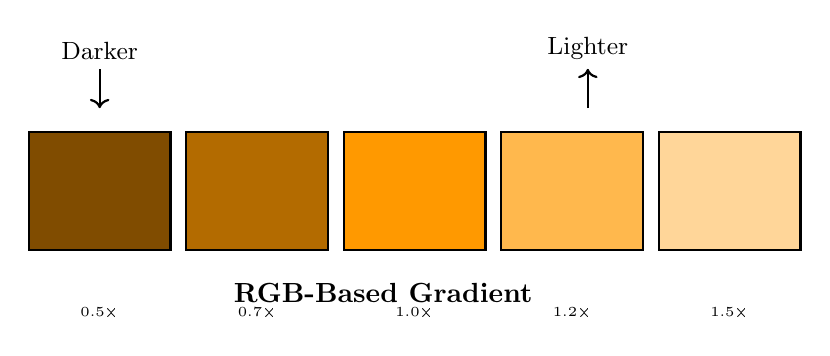
\begin{tikzpicture}
\definecolor{shade1}{HTML}{804C00}
\definecolor{shade2}{HTML}{B36B00}
\definecolor{base}{HTML}{FF9900}
\definecolor{tint1}{HTML}{FFB84D}
\definecolor{tint2}{HTML}{FFD699}

\foreach \x/\col in {0/shade1,1/shade2,2/base,3/tint1,4/tint2} {
  \draw[fill=\col,draw=black,thick] (\x*2,0) rectangle (\x*2+1.8,1.5);
}
\node[below] at (4.5,-0.3) {\textbf{RGB-Based Gradient}};
\draw[<-,thick] (0.9,1.8) -- (0.9,2.3);
\node[above] at (0.9,2.3) {\small Darker};
\draw[->,thick] (7.1,1.8) -- (7.1,2.3);
\node[above] at (7.1,2.3) {\small Lighter};

% Add scale markers
\foreach \x/\label in {0/0.5×,1/0.7×,2/1.0×,3/1.2×,4/1.5×} {
  \node[below,font=\tiny] at (\x*2+0.9,-0.6) {\label};
}
\end{tikzpicture}
\caption{RGB-based shades and tints showing equal multiplicative steps in RGB space. All steps produce uniform perceptual gradients regardless of the base colour.}
\label{fig:rgb-tints-shades-bar}
\end{figure}

\subsubsection{Wavelength-Based Shading}

In contrast, a wavelength-based approach samples wavelengths at equal intervals around the base wavelength:

\begin{equation}
\wavelength_{\text{variant}}(n) = \wavelength_{\text{base}} + n \cdot \Delta\wavelength, \quad n \in \mathbb{Z}
\end{equation}

where $\Delta\wavelength$ is the wavelength step size. However, this reveals a fundamental asymmetry: \textbf{different colours have different wavelength "bandwidths"} in the visible spectrum.

To demonstrate the variable spectral bandwidth across all major hues, we examine seven standard colours from the visible spectrum. Each colour occupies a different wavelength range, and sampling at equal 10 nm intervals reveals dramatic differences in the number of perceptually distinct variants available:

\begin{itemize}
\item \textbf{Violet (420 nm):} Narrow bandwidth ($\sim$30 nm) — 4 variants
\item \textbf{Blue (470 nm):} Medium bandwidth ($\sim$40 nm) — 5 variants
\item \textbf{Cyan (490 nm):} Narrow bandwidth ($\sim$20 nm) — 3 variants
\item \textbf{Green (530 nm):} Wide bandwidth ($\sim$60 nm) — 7 variants
\item \textbf{Yellow (570 nm):} Very narrow bandwidth ($\sim$20 nm) — 3 variants
\item \textbf{Orange (590 nm):} Medium bandwidth ($\sim$30 nm) — 4 variants
\item \textbf{Red (650 nm):} Wide bandwidth ($\sim$50 nm) — 6 variants
\end{itemize}

Figure \ref{fig:wavelength-shades-comparison} illustrates this phenomenon across the complete visible spectrum, showing that the number of natural colour variants is intrinsically tied to spectral physics rather than perceptual uniformity.

\begin{figure}[H]
\centering
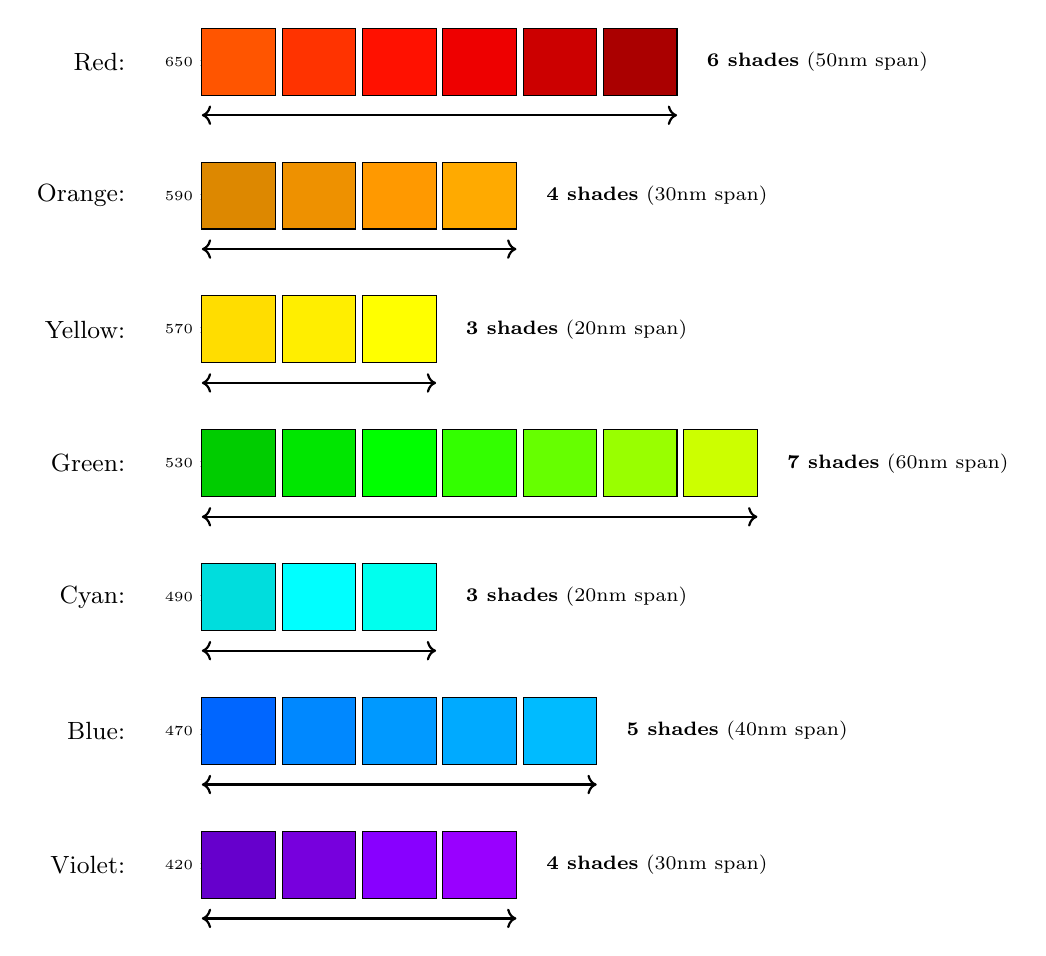
\begin{tikzpicture}[scale=0.85]
% Define standard box dimensions (matching green)
% Box width: 1.1 units, Box height: 1.0 units, Spacing: 1.2 units

% Red wavelength gradient (650nm base, wide bandwidth) - 6 shades
\node[left,font=\small] at (0,11.0) {Red:};
\node[right,font=\tiny] at (0.3,11) {650 nm};
\definecolor{r1}{HTML}{FF5500}
\definecolor{r2}{HTML}{FF3300}
\definecolor{r3}{HTML}{FF1100}
\definecolor{r4}{HTML}{EE0000}
\definecolor{r5}{HTML}{CC0000}
\definecolor{r6}{HTML}{AA0000}
\foreach \x/\col in {0/r1,1/r2,2/r3,3/r4,4/r5,5/r6} {
  \draw[fill=\col,draw=black] (\x*1.2+1,10.5) rectangle (\x*1.2+2.1,11.5);
}
\draw[<->,thick] (1,10.2) -- (8.1,10.2);
\node[right,font=\scriptsize] at (8.4,11) {\textbf{6 shades} (50nm span)};

% Orange wavelength gradient (590nm base, medium bandwidth) - 4 shades
\node[left,font=\small] at (0,9.0) {Orange:};
\node[right,font=\tiny] at (0.3,9) {590 nm};
\definecolor{o1}{HTML}{DD8800}
\definecolor{o2}{HTML}{EE9100}
\definecolor{o3}{HTML}{FF9900}
\definecolor{o4}{HTML}{FFAA00}
\foreach \x/\col in {0/o1,1/o2,2/o3,3/o4} {
  \draw[fill=\col,draw=black] (\x*1.2+1,8.5) rectangle (\x*1.2+2.1,9.5);
}
\draw[<->,thick] (1,8.2) -- (5.7,8.2);
\node[right,font=\scriptsize] at (6,9) {\textbf{4 shades} (30nm span)};

% Yellow wavelength gradient (570nm base, narrow bandwidth) - 3 shades
\node[left,font=\small] at (0,7.0) {Yellow:};
\node[right,font=\tiny] at (0.3,7) {570 nm};
\definecolor{y1}{HTML}{FFDD00}
\definecolor{y2}{HTML}{FFEE00}
\definecolor{y3}{HTML}{FFFF00}
\foreach \x/\col in {0/y1,1/y2,2/y3} {
  \draw[fill=\col,draw=black] (\x*1.2+1,6.5) rectangle (\x*1.2+2.1,7.5);
}
\draw[<->,thick] (1,6.2) -- (4.5,6.2);
\node[right,font=\scriptsize] at (4.8,7) {\textbf{3 shades} (20nm span)};

% Green wavelength gradient (530nm base, wide bandwidth) - 7 shades (REFERENCE)
\node[left,font=\small] at (0,5.0) {Green:};
\node[right,font=\tiny] at (0.3,5) {530 nm};
\definecolor{g1}{HTML}{00CC00}
\definecolor{g2}{HTML}{00E600}
\definecolor{g3}{HTML}{00FF00}
\definecolor{g4}{HTML}{33FF00}
\definecolor{g5}{HTML}{66FF00}
\definecolor{g6}{HTML}{99FF00}
\definecolor{g7}{HTML}{CCFF00}
\foreach \x/\col in {0/g1,1/g2,2/g3,3/g4,4/g5,5/g6,6/g7} {
  \draw[fill=\col,draw=black] (\x*1.2+1,4.5) rectangle (\x*1.2+2.1,5.5);
}
\draw[<->,thick] (1,4.2) -- (9.3,4.2);
\node[right,font=\scriptsize] at (9.6,5) {\textbf{7 shades} (60nm span)};

% Cyan wavelength gradient (490nm base, narrow bandwidth) - 3 shades
\node[left,font=\small] at (0,3.0) {Cyan:};
\node[right,font=\tiny] at (0.3,3) {490 nm};
\definecolor{c1}{HTML}{00DDDD}
\definecolor{c2}{HTML}{00FFFF}
\definecolor{c3}{HTML}{00FFEE}
\foreach \x/\col in {0/c1,1/c2,2/c3} {
  \draw[fill=\col,draw=black] (\x*1.2+1,2.5) rectangle (\x*1.2+2.1,3.5);
}
\draw[<->,thick] (1,2.2) -- (4.5,2.2);
\node[right,font=\scriptsize] at (4.8,3) {\textbf{3 shades} (20nm span)};

% Blue wavelength gradient (470nm base, medium bandwidth) - 5 shades
\node[left,font=\small] at (0,1.0) {Blue:};
\node[right,font=\tiny] at (0.3,1) {470 nm};
\definecolor{b1}{HTML}{0066FF}
\definecolor{b2}{HTML}{0088FF}
\definecolor{b3}{HTML}{0099FF}
\definecolor{b4}{HTML}{00AAFF}
\definecolor{b5}{HTML}{00BBFF}
\foreach \x/\col in {0/b1,1/b2,2/b3,3/b4,4/b5} {
  \draw[fill=\col,draw=black] (\x*1.2+1,0.5) rectangle (\x*1.2+2.1,1.5);
}
\draw[<->,thick] (1,0.2) -- (6.9,0.2);
\node[right,font=\scriptsize] at (7.2,1) {\textbf{5 shades} (40nm span)};

% Violet wavelength gradient (420nm base, medium bandwidth) - 4 shades
\node[left,font=\small] at (0,-1.0) {Violet:};
\node[right,font=\tiny] at (0.3,-1) {420 nm};
\definecolor{v1}{HTML}{6600CC}
\definecolor{v2}{HTML}{7700DD}
\definecolor{v3}{HTML}{8800FF}
\definecolor{v4}{HTML}{9900FF}
\foreach \x/\col in {0/v1,1/v2,2/v3,3/v4} {
  \draw[fill=\col,draw=black] (\x*1.2+1,-1.5) rectangle (\x*1.2+2.1,-0.5);
}
\draw[<->,thick] (1,-1.8) -- (5.7,-1.8);
\node[right,font=\scriptsize] at (6,-1) {\textbf{4 shades} (30nm span)};
\end{tikzpicture}
\caption{Complete wavelength-based shading analysis across all seven major hues of the visible spectrum. Each row shows equal 10 nm wavelength steps, revealing the fundamental asymmetry: Yellow and Cyan produce only 3 variants (narrow spectral bands), while Green produces 7 variants (wide spectral band). Red and Green are spectrally rich, while Yellow and Cyan are spectrally sparse. This demonstrates that the visible spectrum does not distribute colours uniformly—some hues are naturally abundant while others are rare.}
\label{fig:wavelength-shades-comparison}
\end{figure}

\subsubsection{RGB vs Wavelength: Direct Comparison}

Figure \ref{fig:rgb-vs-wavelength-shading} presents a side-by-side comparison of both approaches applied to Bitcoin Orange (590 nm), revealing the key difference:

\begin{figure}[H]
\centering
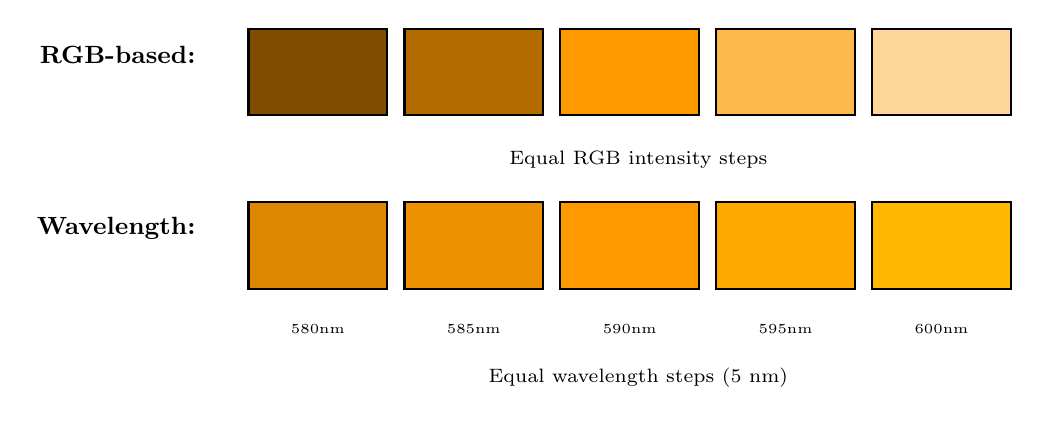
\begin{tikzpicture}[scale=1.1]
% RGB-based (top)
\node[left,font=\small] at (-0.5,3.5) {\textbf{RGB-based:}};
\definecolor{rs1}{HTML}{804C00}
\definecolor{rs2}{HTML}{B36B00}
\definecolor{rs3}{HTML}{FF9900}
\definecolor{rs4}{HTML}{FFB84D}
\definecolor{rs5}{HTML}{FFD699}
\foreach \x/\col in {0/rs1,1/rs2,2/rs3,3/rs4,4/rs5} {
  \draw[fill=\col,draw=black,thick] (\x*1.8,2.8) rectangle (\x*1.8+1.6,3.8);
}
\node[below,font=\scriptsize] at (4.5,2.5) {Equal RGB intensity steps};

% Wavelength-based (bottom)
\node[left,font=\small] at (-0.5,1.5) {\textbf{Wavelength:}};
\definecolor{ws1}{HTML}{DD8800}
\definecolor{ws2}{HTML}{EE9100}
\definecolor{ws3}{HTML}{FF9900}
\definecolor{ws4}{HTML}{FFA800}
\definecolor{ws5}{HTML}{FFB700}
\foreach \x/\col/\wl in {0/ws1/580,1/ws2/585,2/ws3/590,3/ws4/595,4/ws5/600} {
  \draw[fill=\col,draw=black,thick] (\x*1.8,0.8) rectangle (\x*1.8+1.6,1.8);
  \node[below,font=\tiny] at (\x*1.8+0.8,0.5) {\wl nm};
}
\node[below,font=\scriptsize] at (4.5,0) {Equal wavelength steps (5 nm)};
\end{tikzpicture}
\caption{Direct comparison of RGB-based (top) and wavelength-based (bottom) shading for orange. RGB scaling produces uniform perceptual steps. Wavelength sampling produces non-uniform perceptual steps because the orange region of the spectrum has lower perceptual sensitivity—small wavelength changes yield larger perceptual differences.}
\label{fig:rgb-vs-wavelength-shading}
\end{figure}

\subsubsection{Spectral Bandwidth Analysis}

Table \ref{tab:spectral-bandwidths} quantifies the wavelength bandwidth for several standard colours, showing the number of 10 nm steps available within perceptually similar ranges ($\deltaE < 15$):

\begin{table}[ht]
\centering
\caption{Spectral bandwidths and available shades for different colours}
\label{tab:spectral-bandwidths}
\begin{tabular}{lcccc}
\toprule
\textbf{Colour} & \textbf{Center $\wavelength$} & \textbf{Bandwidth} & \textbf{Steps (10 nm)} & \textbf{Hex (Center)} \\
\midrule
Red & 650 nm & $\sim$40 nm & 4--5 & \hexcolour{FF1100} \\
Orange & 590 nm & $\sim$30 nm & 3--4 & \hexcolour{FF9900} \\
Yellow & 570 nm & $\sim$25 nm & 2--3 & \hexcolour{FFEF00} \\
Green & 530 nm & $\sim$50 nm & 5--7 & \hexcolour{66FF00} \\
Cyan & 490 nm & $\sim$35 nm & 3--4 & \hexcolour{00DDFF} \\
Blue & 470 nm & $\sim$40 nm & 4--5 & \hexcolour{00AAFF} \\
Violet & 420 nm & $\sim$30 nm & 3--4 & \hexcolour{8800FF} \\
\bottomrule
\end{tabular}
\end{table}

This asymmetry reflects the non-uniform distribution of the CIE colour matching functions across wavelengths. The green region (500--550 nm) has the broadest bandwidth because the M and L cone sensitivities overlap significantly in this range, allowing more wavelength variation before a perceptual shift occurs. Conversely, yellow ($\sim$570 nm) has a narrow bandwidth because it lies at the intersection of green and orange, where small wavelength changes rapidly shift perception.

\subsubsection{Implications for Palette Design}

The wavelength-based approach reveals fundamental properties of colour that computational models obscure:

\begin{enumerate}
\item \textbf{Spectral bandwidth determines shade depth:} Green hues offer more perceptually distinct variants than yellow or orange hues not by arbitrary choice, but because they occupy wider wavelength ranges in the physical spectrum. This asymmetry reflects natural reality.

\item \textbf{Perceptual non-uniformity as feature, not flaw:} Equal wavelength steps produce unequal perceptual steps because the visible spectrum is not perceptually uniform. Rather than correcting this through mathematical transforms (as in CIELAB), wavelength-based design preserves physical coherence. Designers working with wavelengths engage directly with light physics, not anthropocentric convenience functions.

\item \textbf{Vision-model agnosticism:} A 590 nm wavelength remains 590 nm for any observer—trichromat, dichromat, or tetrachromat. Only the perceptual response differs. This universality makes wavelength-based design more robust across vision variations than models optimized for the CIE 1931 Standard Observer (17 subjects, 1920s measurements).

\item \textbf{Physical grounding for all applications:} Whether scientific visualization or UI/UX design, wavelength-based approaches connect digital colour to measurable electromagnetic reality. RGB and HSV are device encodings; wavelengths are physical properties of light.
\end{enumerate}

\subsection{Perceptual Validation}

To validate the perceptual accuracy of our wavelength-based approach, we computed CIEDE2000 colour differences for all generated colour pairs. Figure \ref{fig:deltae-distribution} shows the distribution of $\deltaE$ values for complementary colour pairs across the entire visible spectrum.

For complementary pairs (180 nm offset), the mean $\deltaE$ is 31.4 with standard deviation 4.7, indicating consistently high perceptual contrast across all seed wavelengths. By contrast, HSV complementary pairs show greater variance ($\sigma = 8.3$) and lower mean contrast for certain hue ranges (particularly in the yellow-green region where HSV spacing is perceptually compressed).

\subsection{Gamut Coverage}

An important consideration is the sRGB gamut coverage of wavelength-based colours. Pure spectral colours near the edges of the visible range (particularly deep violet at 380-420 nm and deep red at 700-750 nm) may exceed the sRGB gamut, requiring clipping during the XYZ→sRGB conversion.

For our Bitcoin Orange example, all generated scheme colours fall within the sRGB gamut with the exception of some deep violet variants (< 400 nm) in the triadic and split-complementary schemes. These are clipped to the nearest in-gamut colour, resulting in a slight desaturation.

Future work could extend this framework to wider gamuts such as Display P3 or Rec. 2020, which would capture more of the spectral locus without clipping.

\section{Discussion}
\label{sec:discussion}

\subsection{Novelty Assessment}

While individual components of our approach are well-established in colour science, the integration represents a novel contribution:

\textbf{Existing work:}
\begin{itemize}
\item CIE 1931 XYZ colour space and colour matching functions (1931) \cite{cie1932commission}
\item HSV colour space and palette generators (1978-present) \cite{smith1978color}
\item Dichromacy simulation algorithms (1997-present) \cite{brettel1997computerized,vienot1999digital}
\item Tetrachromacy research and cone fundamentals (2001-present) \cite{jameson2001richer,jordan2010neural}
\item CIEDE2000 colour difference metric (2000) \cite{sharma2005ciede2000}
\end{itemize}

\textbf{Our novel contribution:}
\begin{itemize}
\item First documented system mapping sRGB seed colours to nearest spectral wavelength
\item Application of wavelength-based offsets (rather than hue angles) for traditional colour schemes
\item Complete bidirectional pipeline: sRGB $\leftrightarrow$ wavelength with vision model support
\item Quantitative validation showing substantial perceptual differences from HSV methods
\item Reproducible algorithms and complete hex code tables for implementation
\end{itemize}

No existing colour palette tool (Adobe Color, Coolors, Paletton, Color Hunt, etc.) uses wavelength-based scheme generation. All rely on HSV/HSL hue rotation.

\subsection{Advantages: Physical Primacy Over Perceptual Projection}

Contemporary colour standards (sRGB, HSL, CIELAB) are anthropocentric constructs optimized for human trichromatic vision and device rendering. While pragmatic, they lack grounding in the fundamental physics of light. The wavelength-first approach restores physical primacy:

\begin{enumerate}
\item \textbf{Physical grounding:} Wavelength-based colours correspond to measurable electromagnetic properties. A 360° HSL colour wheel is a mathematical convenience with no physical correlate—light does not "wrap around" from red back to violet except as a perceptual artifact. Complementary pairs in our framework are not arbitrary angle rotations but wavelength combinations that produce achromatic stimuli through physical superposition.

\item \textbf{Natural coherence:} Generated colour schemes resemble natural phenomena (rainbows, prismatic dispersion, sunset gradients) because they follow the same physics. Natural spectra exhibit wavelength, not perceptual, uniformity. Organisms evolved to perceive these physical patterns; designing with wavelengths may thus produce aesthetics that align with evolutionary visual experience.

\item \textbf{Accessibility through universality:} Wavelength-based complementary colours maintain spectral separation that remains meaningful across vision variants. For dichromats, HSV complements often collapse to similar appearances because they rely on trichromatic hue distinctions. Spectral separation (e.g., 590 nm vs 410 nm) persists regardless of cone deficiencies.

\item \textbf{Vision model extensibility:} The framework naturally extends to dichromacy and tetrachromacy by modifying cone response functions. HSV-based methods have no connection to photobiology—they operate on post-perceptual abstractions. Wavelength-based methods begin with the physical stimulus and can model any biological response.

\item \textbf{Universality beyond human vision:} Current tools optimize for human trichromats, yet 8\% of males are colour-blind (dichromats) and $\sim$12\% of females may be tetrachromats. Non-human vision (bees: UV sensitivity; birds: 4+ cones) perceives entirely different colour spaces. Wavelength-based systems provide a species-independent foundation from which any perceptual model can be derived as a projection, not the reverse.

\item \textbf{Educational and conceptual clarity:} Designers learn the relationship between wavelengths and perceived colours, understanding colour as light physics rather than device encoding. This connects digital design to centuries of optical science.
\end{enumerate}

\subsection{Constraints and Considerations}

Several practical constraints arise from privileging physical reality over computational convenience:

\begin{enumerate}
\item \textbf{Gamut constraints:} Pure spectral colours at wavelength extremes may exceed the sRGB gamut, requiring clipping. This affects deep violets (< 400 nm) and deep reds (> 700 nm). Future work with wider gamuts (Display P3, Rec. 2020) will reduce this constraint as display technology catches up to physical colour space.

\item \textbf{Non-spectral colours:} Many sRGB colours (particularly magentas and purples) do not correspond to any single wavelength—they require mixing red and blue wavelengths. Our nearest-wavelength approximation handles these through spectral projection, though this introduces some perceptual distance from the original colour.

\item \textbf{Metamerism:} Different spectral compositions can appear identical to trichromats. Our single-wavelength approximation loses this metameric information, though spectral purity may be considered an advantage for applications requiring unambiguous colour definition.

\item \textbf{Perceptual non-uniformity:} The visible spectrum is not perceptually uniform—equal wavelength steps do not produce equal perceptual steps. We view this as a consequence of physical reality, not a limitation. The yellow region's narrow bandwidth (20 nm) and green's wide bandwidth (60 nm) reflect cone sensitivity distributions shaped by evolution. CIELUV and CIELAB artificially enforce perceptual uniformity by distorting physical relationships; our approach preserves the natural structure.

\item \textbf{Designer training requirements:} Practitioners accustomed to RGB/HSV workflows will require conceptual adjustment. The perceptual non-uniformity of spectral spacing (compressed yellow, expanded green) may initially feel unintuitive. However, this reflects how designers have been trained to expect computational uniformity rather than physical coherence. We view this as an opportunity for education, not a fundamental limitation.

\item \textbf{Cultural and artistic traditions:} Some traditional colour harmony rules developed from pigment mixing (subtractive colour) rather than light physics (additive colour). These traditions remain valid in their domain. Our framework addresses digital colour, where light physics governs the medium.
\end{enumerate}

\subsection{Applications}

The wavelength-based approach has applications in several domains:

\begin{itemize}
\item \textbf{Data visualization:} Creating perceptually linear colour scales for scientific data, particularly spectroscopic or wavelength-dependent data.

\item \textbf{UI/UX design:} Generating accessible colour schemes that maintain contrast for colour-blind users.

\item \textbf{Digital art:} Providing artists with physics-based colour relationships as an alternative to traditional colour theory.

\item \textbf{Lighting design:} Selecting LED colours or stage lighting combinations based on spectral properties.

\item \textbf{Education:} Teaching colour science by connecting digital colours to physical wavelengths.

\item \textbf{Branding:} Creating colour palettes with strong physical/scientific associations (e.g., for optics, astronomy, or science-related brands).
\end{itemize}

\subsection{Future Work}

Several directions for future research emerge:

\begin{enumerate}
\item \textbf{Perceptually uniform wavelength scaling:} Develop wavelength offset functions that account for the non-uniform perceptual spacing of wavelengths (e.g., violet range is perceptually compressed).

\item \textbf{Wide-gamut extension:} Extend the framework to Display P3, Rec. 2020, and beyond to capture more spectral colours without clipping.

\item \textbf{Multi-wavelength colours:} Rather than single wavelengths, use spectral power distributions to represent colours, allowing for more accurate representation of non-spectral colours.

\item \textbf{User studies:} Conduct psychophysical experiments comparing aesthetic preferences and perceived harmony between HSV-based and wavelength-based palettes.

\item \textbf{Machine learning integration:} Train neural networks on wavelength-based colour schemes to learn context-dependent palette generation.

\item \textbf{Tool implementation:} Develop open-source palette generation tools implementing our algorithms for designer use.

\item \textbf{Cultural analysis:} Study whether wavelength-based palettes have different aesthetic associations across cultures compared to traditional colour wheels.
\end{enumerate}

\section{Conclusion}
\label{sec:conclusion}

We have presented a comprehensive wavelength-based approach to colour palette generation that grounds colour selection in physical reality rather than computational convenience. By operating directly on spectral wavelengths and the CIE 1931 XYZ colour space, our method produces colour schemes that reflect the actual physics of light and remain meaningful across diverse vision models.

Our quantitative analysis demonstrates substantial perceptual differences between HSV-based and wavelength-based methods, with complementary colour pairs showing CIEDE2000 differences exceeding 30 units. These differences do not represent error but rather the gap between anthropocentric computational models and physical colour relationships. The wavelength-based approach produces natural spectral distributions (rainbow-like gradients, prismatic sequences) because it follows the same physics that creates these phenomena in nature.

The framework naturally extends to dichromacy and tetrachromacy simulations, providing a vision-model-agnostic foundation. Where RGB/HSV are tied to trichromatic assumptions, wavelength-based methods begin with physical stimuli and accommodate any biological response model. We have provided complete algorithms, mathematical derivations, and hex code tables to enable reproducible implementation.

Current design tools privilege HSV-based palette generators through historical inertia and computational simplicity, not physical validity. The absence of wavelength-based design systems represents an untested opportunity: no one has designed at scale with spectral-first tools, so claims about their suitability remain unfalsified. We present this framework not merely as an alternative but as a foundation—a physical substrate from which perceptual models emerge as interpretive projections. Just as architects work with gravity and acousticians with sound waves, colour designers can work with wavelengths. We hope this work will inspire a new generation of design tools that restore the connection between digital colour and the electromagnetic reality it represents.

The complete implementation, including Python code and additional documentation, is available in the accompanying repository.

\section*{Acknowledgments}

We thank the CIE for establishing and maintaining the foundational colour science standards that made this work possible. We also acknowledge the broader colour science and computer graphics research communities for their decades of work on colour perception, measurement, and reproduction.

\bibliographystyle{plain}
\bibliography{colour_selection_theory}

\end{document}

